% Options for packages loaded elsewhere
\PassOptionsToPackage{unicode}{hyperref}
\PassOptionsToPackage{hyphens}{url}
%
\documentclass[
]{article}
\usepackage{lmodern}
\usepackage{amsmath}
\usepackage{ifxetex,ifluatex}
\ifnum 0\ifxetex 1\fi\ifluatex 1\fi=0 % if pdftex
  \usepackage[T1]{fontenc}
  \usepackage[utf8]{inputenc}
  \usepackage{textcomp} % provide euro and other symbols
  \usepackage{amssymb}
\else % if luatex or xetex
  \usepackage{unicode-math}
  \defaultfontfeatures{Scale=MatchLowercase}
  \defaultfontfeatures[\rmfamily]{Ligatures=TeX,Scale=1}
\fi
% Use upquote if available, for straight quotes in verbatim environments
\IfFileExists{upquote.sty}{\usepackage{upquote}}{}
\IfFileExists{microtype.sty}{% use microtype if available
  \usepackage[]{microtype}
  \UseMicrotypeSet[protrusion]{basicmath} % disable protrusion for tt fonts
}{}
\makeatletter
\@ifundefined{KOMAClassName}{% if non-KOMA class
  \IfFileExists{parskip.sty}{%
    \usepackage{parskip}
  }{% else
    \setlength{\parindent}{0pt}
    \setlength{\parskip}{6pt plus 2pt minus 1pt}}
}{% if KOMA class
  \KOMAoptions{parskip=half}}
\makeatother
\usepackage{xcolor}
\IfFileExists{xurl.sty}{\usepackage{xurl}}{} % add URL line breaks if available
\IfFileExists{bookmark.sty}{\usepackage{bookmark}}{\usepackage{hyperref}}
\hypersetup{
  pdftitle={HiTMaP},
  hidelinks,
  pdfcreator={LaTeX via pandoc}}
\urlstyle{same} % disable monospaced font for URLs
\usepackage[margin=1in]{geometry}
\usepackage{color}
\usepackage{fancyvrb}
\newcommand{\VerbBar}{|}
\newcommand{\VERB}{\Verb[commandchars=\\\{\}]}
\DefineVerbatimEnvironment{Highlighting}{Verbatim}{commandchars=\\\{\}}
% Add ',fontsize=\small' for more characters per line
\usepackage{framed}
\definecolor{shadecolor}{RGB}{248,248,248}
\newenvironment{Shaded}{\begin{snugshade}}{\end{snugshade}}
\newcommand{\AlertTok}[1]{\textcolor[rgb]{0.94,0.16,0.16}{#1}}
\newcommand{\AnnotationTok}[1]{\textcolor[rgb]{0.56,0.35,0.01}{\textbf{\textit{#1}}}}
\newcommand{\AttributeTok}[1]{\textcolor[rgb]{0.77,0.63,0.00}{#1}}
\newcommand{\BaseNTok}[1]{\textcolor[rgb]{0.00,0.00,0.81}{#1}}
\newcommand{\BuiltInTok}[1]{#1}
\newcommand{\CharTok}[1]{\textcolor[rgb]{0.31,0.60,0.02}{#1}}
\newcommand{\CommentTok}[1]{\textcolor[rgb]{0.56,0.35,0.01}{\textit{#1}}}
\newcommand{\CommentVarTok}[1]{\textcolor[rgb]{0.56,0.35,0.01}{\textbf{\textit{#1}}}}
\newcommand{\ConstantTok}[1]{\textcolor[rgb]{0.00,0.00,0.00}{#1}}
\newcommand{\ControlFlowTok}[1]{\textcolor[rgb]{0.13,0.29,0.53}{\textbf{#1}}}
\newcommand{\DataTypeTok}[1]{\textcolor[rgb]{0.13,0.29,0.53}{#1}}
\newcommand{\DecValTok}[1]{\textcolor[rgb]{0.00,0.00,0.81}{#1}}
\newcommand{\DocumentationTok}[1]{\textcolor[rgb]{0.56,0.35,0.01}{\textbf{\textit{#1}}}}
\newcommand{\ErrorTok}[1]{\textcolor[rgb]{0.64,0.00,0.00}{\textbf{#1}}}
\newcommand{\ExtensionTok}[1]{#1}
\newcommand{\FloatTok}[1]{\textcolor[rgb]{0.00,0.00,0.81}{#1}}
\newcommand{\FunctionTok}[1]{\textcolor[rgb]{0.00,0.00,0.00}{#1}}
\newcommand{\ImportTok}[1]{#1}
\newcommand{\InformationTok}[1]{\textcolor[rgb]{0.56,0.35,0.01}{\textbf{\textit{#1}}}}
\newcommand{\KeywordTok}[1]{\textcolor[rgb]{0.13,0.29,0.53}{\textbf{#1}}}
\newcommand{\NormalTok}[1]{#1}
\newcommand{\OperatorTok}[1]{\textcolor[rgb]{0.81,0.36,0.00}{\textbf{#1}}}
\newcommand{\OtherTok}[1]{\textcolor[rgb]{0.56,0.35,0.01}{#1}}
\newcommand{\PreprocessorTok}[1]{\textcolor[rgb]{0.56,0.35,0.01}{\textit{#1}}}
\newcommand{\RegionMarkerTok}[1]{#1}
\newcommand{\SpecialCharTok}[1]{\textcolor[rgb]{0.00,0.00,0.00}{#1}}
\newcommand{\SpecialStringTok}[1]{\textcolor[rgb]{0.31,0.60,0.02}{#1}}
\newcommand{\StringTok}[1]{\textcolor[rgb]{0.31,0.60,0.02}{#1}}
\newcommand{\VariableTok}[1]{\textcolor[rgb]{0.00,0.00,0.00}{#1}}
\newcommand{\VerbatimStringTok}[1]{\textcolor[rgb]{0.31,0.60,0.02}{#1}}
\newcommand{\WarningTok}[1]{\textcolor[rgb]{0.56,0.35,0.01}{\textbf{\textit{#1}}}}
\usepackage{graphicx}
\makeatletter
\def\maxwidth{\ifdim\Gin@nat@width>\linewidth\linewidth\else\Gin@nat@width\fi}
\def\maxheight{\ifdim\Gin@nat@height>\textheight\textheight\else\Gin@nat@height\fi}
\makeatother
% Scale images if necessary, so that they will not overflow the page
% margins by default, and it is still possible to overwrite the defaults
% using explicit options in \includegraphics[width, height, ...]{}
\setkeys{Gin}{width=\maxwidth,height=\maxheight,keepaspectratio}
% Set default figure placement to htbp
\makeatletter
\def\fps@figure{htbp}
\makeatother
\setlength{\emergencystretch}{3em} % prevent overfull lines
\providecommand{\tightlist}{%
  \setlength{\itemsep}{0pt}\setlength{\parskip}{0pt}}
\setcounter{secnumdepth}{-\maxdimen} % remove section numbering
\ifluatex
  \usepackage{selnolig}  % disable illegal ligatures
\fi
\newlength{\cslhangindent}
\setlength{\cslhangindent}{1.5em}
\newlength{\csllabelwidth}
\setlength{\csllabelwidth}{3em}
\newenvironment{CSLReferences}[2] % #1 hanging-ident, #2 entry spacing
 {% don't indent paragraphs
  \setlength{\parindent}{0pt}
  % turn on hanging indent if param 1 is 1
  \ifodd #1 \everypar{\setlength{\hangindent}{\cslhangindent}}\ignorespaces\fi
  % set entry spacing
  \ifnum #2 > 0
  \setlength{\parskip}{#2\baselineskip}
  \fi
 }%
 {}
\usepackage{calc}
\newcommand{\CSLBlock}[1]{#1\hfill\break}
\newcommand{\CSLLeftMargin}[1]{\parbox[t]{\csllabelwidth}{#1}}
\newcommand{\CSLRightInline}[1]{\parbox[t]{\linewidth - \csllabelwidth}{#1}\break}
\newcommand{\CSLIndent}[1]{\hspace{\cslhangindent}#1}

\title{HiTMaP}
\author{}
\date{\vspace{-2.5em}}

\begin{document}
\maketitle

-- An R package of High-resolution Informatics Toolbox for Maldi-imaging
Proteomics

\hypertarget{package-installation}{%
\subsection{Package installation}\label{package-installation}}

This is an tutorial for use of HiTMaP (An R package of High-resolution
Informatics Toolbox for Maldi-imaging Proteomics). To access the
software use the installation codes as below:

\hypertarget{installation-from-docker-image}{%
\subsubsection{Installation from Docker
image}\label{installation-from-docker-image}}

HiTMaP has been encapsulated as an docker image for each release. User
can download the latest version by using the code as below.

\begin{Shaded}
\begin{Highlighting}[]
\ExtensionTok{docker}\NormalTok{ login {-}{-}username mashuoa}
\ExtensionTok{0a9da0ae{-}8d7b{-}4e11{-}8587{-}be46e21ee937}
\ExtensionTok{docker}\NormalTok{ pull mashuoa/hitmap}
\end{Highlighting}
\end{Shaded}

Setup and run the container:

\begin{Shaded}
\begin{Highlighting}[]
\CommentTok{\#for windows user, run the image with a local user\textbackslash{}Documents\textbackslash{}expdata folder mapped to the docker container:}
\ExtensionTok{docker}\NormalTok{ run {-}{-}name hitmap {-}v \%userprofile\%\textbackslash{}Documents\textbackslash{}expdata:/root/expdata {-}a stdin {-}a stdout {-}i {-}t mashuoa/hitmap /bin/bash }

\CommentTok{\#for linux user, run the image with a local user/expdata folder mapped to the docker container:}
\ExtensionTok{docker}\NormalTok{ run {-}{-}name hitmap {-}v \textasciitilde{}/expdata:/root/expdata {-}a stdin {-}a stdout {-}i {-}t mashuoa/hitmap /bin/bash }

\CommentTok{\#Restart the shell }
\ExtensionTok{docker}\NormalTok{ container exec {-}it hitmap /bin/bash}

\CommentTok{\#Run R console}
\ExtensionTok{R}
\end{Highlighting}
\end{Shaded}

If You are using docker GUI, pull the docker image using the codes above
and follow the image as below to setup the container.

\begin{figure}
\centering
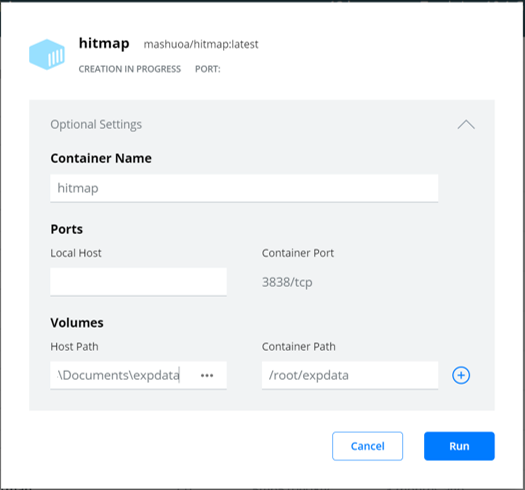
\includegraphics{Resource/docker_gui_setting.png}
\caption{Docker GUI setting}
\end{figure}

\hypertarget{installation-code-for-r-console-installation}{%
\subsubsection{Installation code for R console
installation}\label{installation-code-for-r-console-installation}}

\begin{Shaded}
\begin{Highlighting}[]
\CommentTok{\#install the git package}
\FunctionTok{install.packages}\NormalTok{(}\StringTok{"remotes"}\NormalTok{)}
\FunctionTok{install.packages}\NormalTok{(}\StringTok{"devtools"}\NormalTok{)}
\CommentTok{\#library(devtools)}
\FunctionTok{library}\NormalTok{(remotes)}
\FunctionTok{Sys.setenv}\NormalTok{(}\StringTok{"R\_REMOTES\_NO\_ERRORS\_FROM\_WARNINGS"} \OtherTok{=} \StringTok{"true"}\NormalTok{)}
\NormalTok{remotes}\SpecialCharTok{::}\FunctionTok{install\_github}\NormalTok{(}\StringTok{"MASHUOA/HiTMaP"}\NormalTok{,}\AttributeTok{auth\_token =}\StringTok{"cf6d877f8b6ada1865987b13f9e9996c1883014a"}\NormalTok{,}\AttributeTok{force=}\NormalTok{T)}
\DecValTok{3}
\NormalTok{no}
\CommentTok{\#Update all dependencies}
\NormalTok{BiocManager}\SpecialCharTok{::}\FunctionTok{install}\NormalTok{(}\AttributeTok{ask =}\NormalTok{ F)}
\NormalTok{yes}
\FunctionTok{library}\NormalTok{(HiTMaP)}
\end{Highlighting}
\end{Shaded}

For windows users, Rtools
(\emph{\url{https://cran.r-project.org/bin/windows/Rtools/}}) is
required.

\hypertarget{codes-for-linux-os-building-enviornment}{%
\subsubsection{Codes for Linux OS building
enviornment}\label{codes-for-linux-os-building-enviornment}}

Run the codes as below to enable the required components in Linux
console.

\begin{Shaded}
\begin{Highlighting}[]
\FunctionTok{sudo}\NormalTok{ apt{-}get install tcl{-}dev tk{-}dev}
\FunctionTok{sudo}\NormalTok{ apt{-}get install r{-}cran{-}ncdf4}
\ExtensionTok{apt{-}get}\NormalTok{ install libz{-}dev}
\FunctionTok{sudo}\NormalTok{ apt install libxml2{-}dev}
\FunctionTok{sudo}\NormalTok{ apt install libssl{-}dev}
\FunctionTok{sudo}\NormalTok{ apt install libcurl4{-}openssl{-}dev}
\FunctionTok{sudo}\NormalTok{ apt{-}get install libnss{-}winbind winbind}
\FunctionTok{sudo}\NormalTok{ apt install dirmngr gnupg apt{-}transport{-}https ca{-}certificates software{-}properties{-}common}
\FunctionTok{sudo}\NormalTok{ apt{-}key adv {-}{-}keyserver keyserver.ubuntu.com {-}{-}recv{-}keys}
\FunctionTok{sudo}\NormalTok{ add{-}apt{-}repository }\StringTok{\textquotesingle{}deb https://cloud.r{-}project.org/bin/linux/ubuntu focal{-}cran40/\textquotesingle{}}
\FunctionTok{sudo}\NormalTok{ apt{-}cache policy r{-}base}
\ExtensionTok{apt{-}get}\NormalTok{ purge r{-}base}
\FunctionTok{sudo}\NormalTok{ apt{-}get install r{-}base{-}core=}\StringTok{"4.0.2{-}1.2004.0"}
\FunctionTok{sudo}\NormalTok{ apt{-}get install libmagick++{-}dev}
\ExtensionTok{apt{-}get}\NormalTok{ install libfftw3{-}dev}
\FunctionTok{sudo}\NormalTok{ apt{-}get install r{-}base{-}dev texlive{-}full}
\FunctionTok{sudo}\NormalTok{ apt{-}get install libudunits2{-}dev}
\FunctionTok{sudo}\NormalTok{ apt{-}get install libgdal{-}dev}
\end{Highlighting}
\end{Shaded}

\hypertarget{codes-for-mac-os-building-enviornment}{%
\subsubsection{Codes for Mac OS building
enviornment}\label{codes-for-mac-os-building-enviornment}}

You may need to update the Xcode. Go to your Mac OS terminal and input:

\begin{Shaded}
\begin{Highlighting}[]
\ExtensionTok{xcode{-}select}\NormalTok{ {-}{-}install}
\end{Highlighting}
\end{Shaded}

You'll then receive: \emph{xcode-select: note: install requested for
command line developer tools} You will be prompted at this point in a
window to update Xcode Command Line tools.

You may also need to install the X11.app and tcl/tk support for Mac
system:

\begin{itemize}
\item
  X11.app: \url{https://www.xquartz.org/}
\item
  Use the following link to download and install the correct tcltk
  package for your OS version.
  \url{https://cran.r-project.org/bin/macosx/tools/}
\end{itemize}

\hypertarget{example-data}{%
\subsection{Example data}\label{example-data}}

The HitMaP comes with a series of Maildi imaging data sets acquired from
either FT-ICR or TOF. By the following codes, you can download these raw
data set into a local folder.

You can download the example file manually through this link:
``\url{https://github.com/MASHUOA/HiTMaP/releases/download/1.0/Data.tar.gz}''

Or download the files in a R console:

\begin{Shaded}
\begin{Highlighting}[]
\ControlFlowTok{if}\NormalTok{(}\SpecialCharTok{!}\FunctionTok{require}\NormalTok{(piggyback)) }\FunctionTok{install.packages}\NormalTok{(}\StringTok{"piggyback"}\NormalTok{)}
\FunctionTok{library}\NormalTok{(piggyback)}

\FunctionTok{Sys.setenv}\NormalTok{(}\AttributeTok{GITHUB\_TOKEN=}\StringTok{"cf6d877f8b6ada1865987b13f9e9996c1883014a"}\NormalTok{)}

\CommentTok{\#made sure that this folder has enough space}
\NormalTok{wd}\OtherTok{=}\StringTok{"\textasciitilde{}/expdata/"}
\FunctionTok{dir.create}\NormalTok{(wd)}
\FunctionTok{setwd}\NormalTok{(wd)}
\FunctionTok{pb\_download}\NormalTok{(}\StringTok{"Data.tar.gz"}\NormalTok{, }\AttributeTok{repo =} \StringTok{"MASHUOA/HiTMaP"}\NormalTok{, }\AttributeTok{dest =} \StringTok{"."}\NormalTok{)}
\FunctionTok{untar}\NormalTok{(}\StringTok{\textquotesingle{}Data.tar.gz\textquotesingle{}}\NormalTok{,}\AttributeTok{exdir =}\StringTok{"."}\NormalTok{,  }\AttributeTok{tar=}\StringTok{"tar"}\NormalTok{)}

\CommentTok{\#unlink(\textquotesingle{}Data.tar.gz\textquotesingle{})}
\FunctionTok{list.dirs}\NormalTok{()}
\end{Highlighting}
\end{Shaded}

The example file contains three folder for three IMS dataset,
configuration files, and the fasta database, respectively:
\emph{``./Bovinlens\_Trypsin\_FT'' ``./MouseBrain\_Trypsin\_FT''
``./Peptide\_calibrants\_FT''}

\hypertarget{proteomics-identification-on-maldi-imaging-data-file}{%
\subsection{Proteomics identification on Maldi imaging data
file}\label{proteomics-identification-on-maldi-imaging-data-file}}

Now the HiTMaP is upon running. You could build the candidate list of
your target proteome and perform image identification by using the
function as below:

\begin{Shaded}
\begin{Highlighting}[]
\CommentTok{\#creat candidate list}
\FunctionTok{library}\NormalTok{(HiTMaP)}
\CommentTok{\#set project folder that contains imzML, .ibd and fasta files}
\CommentTok{\#wd=paste0(file.path(path.package(package="HiTMaP")),"/data/")}
\CommentTok{\#set a series of imzML files to be processed}
\NormalTok{datafile}\OtherTok{=}\FunctionTok{c}\NormalTok{(}\StringTok{"Bovinlens\_Trypsin\_FT/Bovin\_lens.imzML"}\NormalTok{)}
\NormalTok{wd}\OtherTok{=}\StringTok{"\textasciitilde{}/expdata/"}


\FunctionTok{imaging\_identification}\NormalTok{(}
\CommentTok{\#==============Choose the imzml raw data file(s) to process  make sure the fasta file in the same folder}
               \AttributeTok{datafile=}\FunctionTok{paste0}\NormalTok{(wd,datafile),}
               \AttributeTok{threshold=}\FloatTok{0.005}\NormalTok{, }
               \AttributeTok{ppm=}\DecValTok{5}\NormalTok{,}
               \AttributeTok{FDR\_cutoff =} \FloatTok{0.05}\NormalTok{,}
\CommentTok{\#==============specify the digestion enzyme specificity}
               \AttributeTok{Digestion\_site=}\StringTok{"trypsin"}\NormalTok{,}
\CommentTok{\#==============specify the range of missed Cleavages}
               \AttributeTok{missedCleavages=}\DecValTok{0}\SpecialCharTok{:}\DecValTok{1}\NormalTok{,}
\CommentTok{\#==============Set the target fasta file}
               \AttributeTok{Fastadatabase=}\StringTok{"uniprot{-}bovin.fasta"}\NormalTok{,}
\CommentTok{\#==============Set the possible adducts and fixed modifications}
               \AttributeTok{adducts=}\FunctionTok{c}\NormalTok{(}\StringTok{"M+H"}\NormalTok{),}
               \AttributeTok{Modifications=}\FunctionTok{list}\NormalTok{(}\AttributeTok{fixed=}\ConstantTok{NULL}\NormalTok{,}\AttributeTok{fixmod\_position=}\ConstantTok{NULL}\NormalTok{,}\AttributeTok{variable=}\ConstantTok{NULL}\NormalTok{,}\AttributeTok{varmod\_position=}\ConstantTok{NULL}\NormalTok{),}
\CommentTok{\#==============The decoy mode: could be one of the "adducts", "elements" or "isotope"}
               \AttributeTok{Decoy\_mode =} \StringTok{"isotope"}\NormalTok{,}
               \AttributeTok{use\_previous\_candidates=}\NormalTok{F,}
               \AttributeTok{output\_candidatelist=}\NormalTok{T,}
\CommentTok{\#==============The pre{-}processing param}
               \AttributeTok{preprocess=}\FunctionTok{list}\NormalTok{(}\AttributeTok{force\_preprocess=}\ConstantTok{TRUE}\NormalTok{,}
                               \AttributeTok{use\_preprocessRDS=}\ConstantTok{TRUE}\NormalTok{,}
                               \AttributeTok{smoothSignal=}\FunctionTok{list}\NormalTok{(}\AttributeTok{method=}\StringTok{"gaussian"}\NormalTok{),}
                               \AttributeTok{reduceBaseline=}\FunctionTok{list}\NormalTok{(}\AttributeTok{method=}\StringTok{"locmin"}\NormalTok{),}
                               \AttributeTok{peakPick=}\FunctionTok{list}\NormalTok{(}\AttributeTok{method=}\StringTok{"adaptive"}\NormalTok{),}
                               \AttributeTok{peakAlign=}\FunctionTok{list}\NormalTok{(}\AttributeTok{tolerance=}\NormalTok{ppm, }\AttributeTok{units=}\StringTok{"ppm"}\NormalTok{),}
                               \AttributeTok{normalize=}\FunctionTok{list}\NormalTok{(}\AttributeTok{method=}\FunctionTok{c}\NormalTok{(}\StringTok{"rms"}\NormalTok{,}\StringTok{"tic"}\NormalTok{,}\StringTok{"reference"}\NormalTok{)[}\DecValTok{1}\NormalTok{],}\AttributeTok{mz=}\DecValTok{1}\NormalTok{)),}
\CommentTok{\#==============Set the parameters for image segmentation}
               \AttributeTok{spectra\_segments\_per\_file=}\DecValTok{4}\NormalTok{,}
               \AttributeTok{Segmentation=}\StringTok{"spatialKMeans"}\NormalTok{,}
               \AttributeTok{Smooth\_range=}\DecValTok{1}\NormalTok{,}
               \AttributeTok{Virtual\_segmentation=}\ConstantTok{FALSE}\NormalTok{,}
               \AttributeTok{Virtual\_segmentation\_rankfile=}\ConstantTok{NULL}\NormalTok{,}
\CommentTok{\#==============Set the Score method for hi{-}resolution isotopic pattern matching}
               \AttributeTok{score\_method=}\StringTok{"SQRTP"}\NormalTok{,}
               \AttributeTok{peptide\_ID\_filter=}\DecValTok{2}\NormalTok{,}
\CommentTok{\#==============Summarise the protein and peptide features across the project the result can be found at the summary folder}
               \AttributeTok{Protein\_feature\_summary=}\ConstantTok{TRUE}\NormalTok{,}
               \AttributeTok{Peptide\_feature\_summary=}\ConstantTok{TRUE}\NormalTok{,}
               \AttributeTok{Region\_feature\_summary=}\ConstantTok{TRUE}\NormalTok{,}
\CommentTok{\#==============The parameters for Cluster imaging. Specify the annotations of interest, the program will perform a case{-}insensitive search on the result file, extract the protein(s) of interest and plot them in the cluster imaging mode}
               \AttributeTok{plot\_cluster\_image\_grid=}\ConstantTok{FALSE}\NormalTok{,}
               \AttributeTok{ClusterID\_colname=}\StringTok{"Protein"}\NormalTok{,}
               \AttributeTok{componentID\_colname=}\StringTok{"Peptide"}\NormalTok{,}
               \AttributeTok{Protein\_desc\_of\_interest=}\FunctionTok{c}\NormalTok{(}\StringTok{"Crystallin"}\NormalTok{,}\StringTok{"Actin"}\NormalTok{),}
               \AttributeTok{Rotate\_IMG=}\ConstantTok{NULL}\NormalTok{,}
\NormalTok{               )}
\end{Highlighting}
\end{Shaded}

\hypertarget{project-folder-and-result-structure}{%
\subsection{Project folder and result
structure}\label{project-folder-and-result-structure}}

In the above function, You have performed proteomics analysis of the
sample data file. It is a tryptic Bovin lens MALDI-imaging file which is
acquired on an FT-ICR MS. The function will take the selected data
files' root directory as the project folder. In this example, the
project folder will be:

\begin{Shaded}
\begin{Highlighting}[]
\FunctionTok{library}\NormalTok{(HiTMaP)}
\NormalTok{wd}\OtherTok{=}\FunctionTok{paste0}\NormalTok{(}\StringTok{"D:}\SpecialCharTok{\textbackslash{}\textbackslash{}}\StringTok{GITHUB LFS}\SpecialCharTok{\textbackslash{}\textbackslash{}}\StringTok{HiTMaP{-}Data}\SpecialCharTok{\textbackslash{}\textbackslash{}}\StringTok{inst"}\NormalTok{,}\StringTok{"/data/Bovinlens\_Trypsin\_FT/"}\NormalTok{)}
\CommentTok{\#set a series of imzML files to be processed}
\NormalTok{datafile}\OtherTok{=}\FunctionTok{c}\NormalTok{(}\StringTok{"Bovin\_lens"}\NormalTok{)}
\NormalTok{wd}
\end{Highlighting}
\end{Shaded}

\begin{verbatim}
## [1] "D:\\GITHUB LFS\\HiTMaP-Data\\inst/data/Bovinlens_Trypsin_FT/"
\end{verbatim}

After the whole identification process, we will get two types of
sub-folders in the project folder:

\begin{Shaded}
\begin{Highlighting}[]
\FunctionTok{list.dirs}\NormalTok{(wd, }\AttributeTok{recursive=}\ConstantTok{FALSE}\NormalTok{)}
\end{Highlighting}
\end{Shaded}

\begin{verbatim}
## [1] "D:\\GITHUB LFS\\HiTMaP-Data\\inst/data/Bovinlens_Trypsin_FT//Bovin_lens ID" 
## [2] "D:\\GITHUB LFS\\HiTMaP-Data\\inst/data/Bovinlens_Trypsin_FT//Summary folder"
\end{verbatim}

\begin{enumerate}
\def\labelenumi{\arabic{enumi}.}
\tightlist
\item
  The one which has an identical name to an input data file contains the
  identification result of that input:

  \begin{itemize}
  \tightlist
  \item
    the protein and peptides list of each segmentation region
  \item
    the PMF matching plot of each segmentation
  \item
    the image that indicates segmentations' boundary (applies to either
    K-mean segmentation (powered by Cardinal) or manually defined
    segmentation)
  \item
    folders of each region contains the detailed identification process,
    FDR plots and isotopic pattern matching plots
  \end{itemize}
\item
  ``Summary folder'' contains:

  \begin{itemize}
  \tightlist
  \item
    the identification summary of protein and peptides across all the
    data
  \item
    the candidate list of all possible proteins and peptides (if
    \emph{use\_previous\_candidates} is set as \textbf{TRUE})
  \item
    the Cluster imaging files of the protein of interest
  \end{itemize}
\end{enumerate}

\hypertarget{identification-result-visulasation-and-interpretation}{%
\subsection{Identification result visulasation and
interpretation}\label{identification-result-visulasation-and-interpretation}}

Now we could visualize the result by the following functions:

To check the segmentation result over the sample, you need got to each
data file ID folder and find the ``spatialKMeans\_image\_plot.png'' (if
you are using the spatial K-means method for segmentation.)

\begin{Shaded}
\begin{Highlighting}[]
\FunctionTok{library}\NormalTok{(magick)}
\end{Highlighting}
\end{Shaded}

\begin{verbatim}
## Warning: package 'magick' was built under R version 4.0.3
\end{verbatim}

\begin{verbatim}
## Linking to ImageMagick 6.9.11.34
## Enabled features: cairo, freetype, fftw, ghostscript, lcms, pango, rsvg, webp
## Disabled features: fontconfig, x11
\end{verbatim}

\begin{Shaded}
\begin{Highlighting}[]
\NormalTok{p}\OtherTok{\textless{}{-}}\FunctionTok{image\_read}\NormalTok{(}\FunctionTok{paste0}\NormalTok{(wd,datafile,}\StringTok{" ID/spatialKMeans\_image\_plot.png"}\NormalTok{))}
\FunctionTok{print}\NormalTok{(p)}
\end{Highlighting}
\end{Shaded}

\begin{verbatim}
##   format width height colorspace matte filesize density
## 1    PNG  1024   2640       sRGB FALSE    30726   72x72
\end{verbatim}

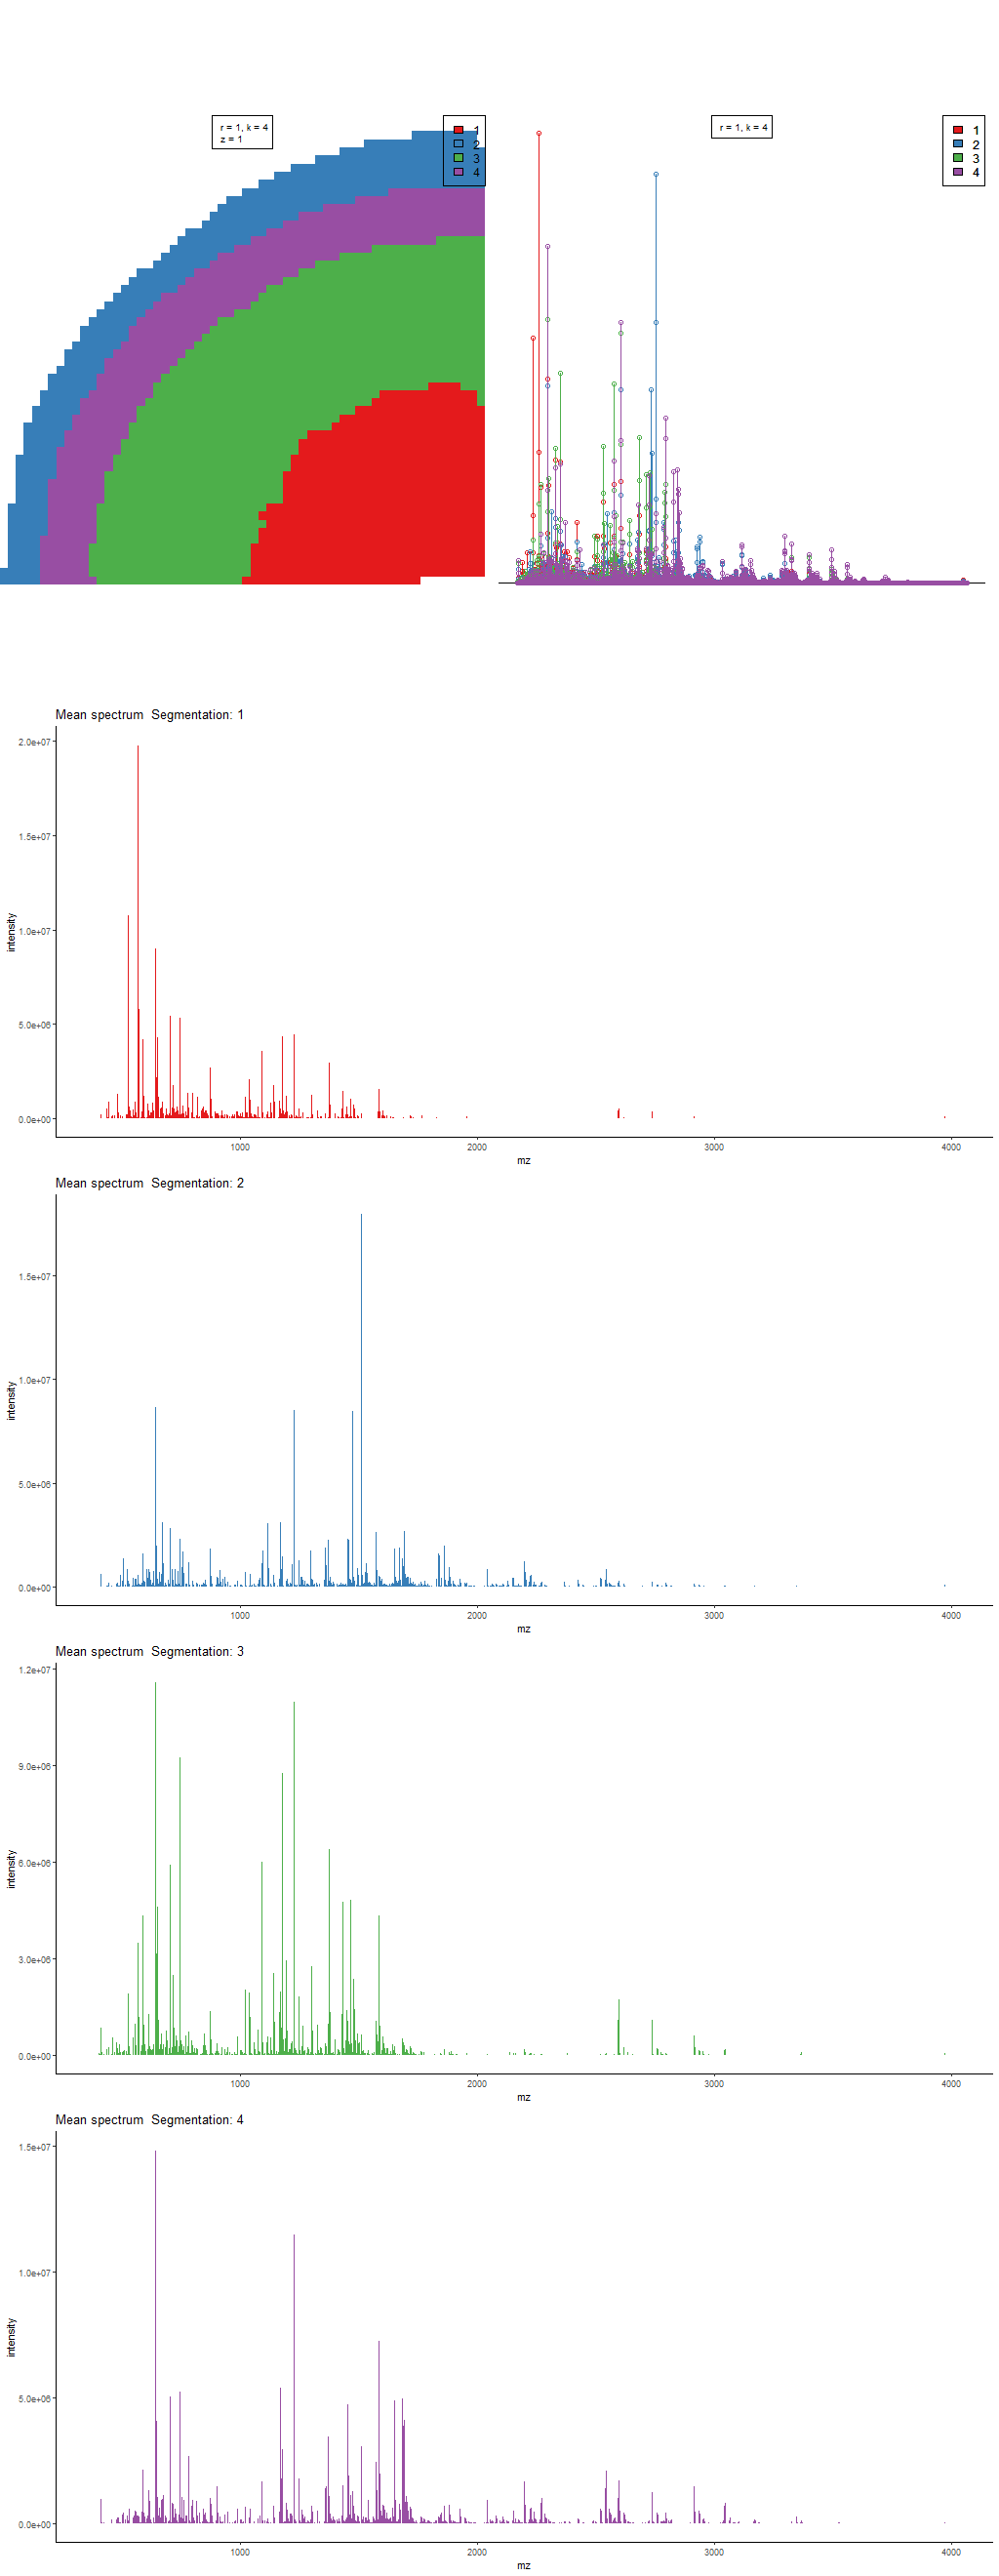
\includegraphics[width=14.22in]{README_files/figure-latex/VisulazeKmean-1}

The pixels in image data now has been categorized into five regions
according to the initial setting of segmentation
(\emph{spectra\_segments\_per\_file=5}). The rainbow shaped bovine lens
segmentation image (on the left panel) shows a unique statistical
classification based on the mz features of each region (on the right
panel).

The identification will take place on the \textbf{mean spectra} of each
region. To check the peptide mass fingerprint (PMF) matching quality,
you could locate the PMF spectrum matching plot of each individual
region.

\begin{Shaded}
\begin{Highlighting}[]
\FunctionTok{library}\NormalTok{(magick)}
\NormalTok{p\_pmf}\OtherTok{\textless{}{-}}\FunctionTok{image\_read}\NormalTok{(}\FunctionTok{paste0}\NormalTok{(wd,datafile,}\StringTok{" ID/Bovin\_lens 3PMF spectrum match.png"}\NormalTok{))}
\FunctionTok{print}\NormalTok{(p\_pmf)}
\end{Highlighting}
\end{Shaded}

\begin{verbatim}
##   format width height colorspace matte filesize density
## 1    PNG  1980   1080       sRGB FALSE    17664   72x72
\end{verbatim}

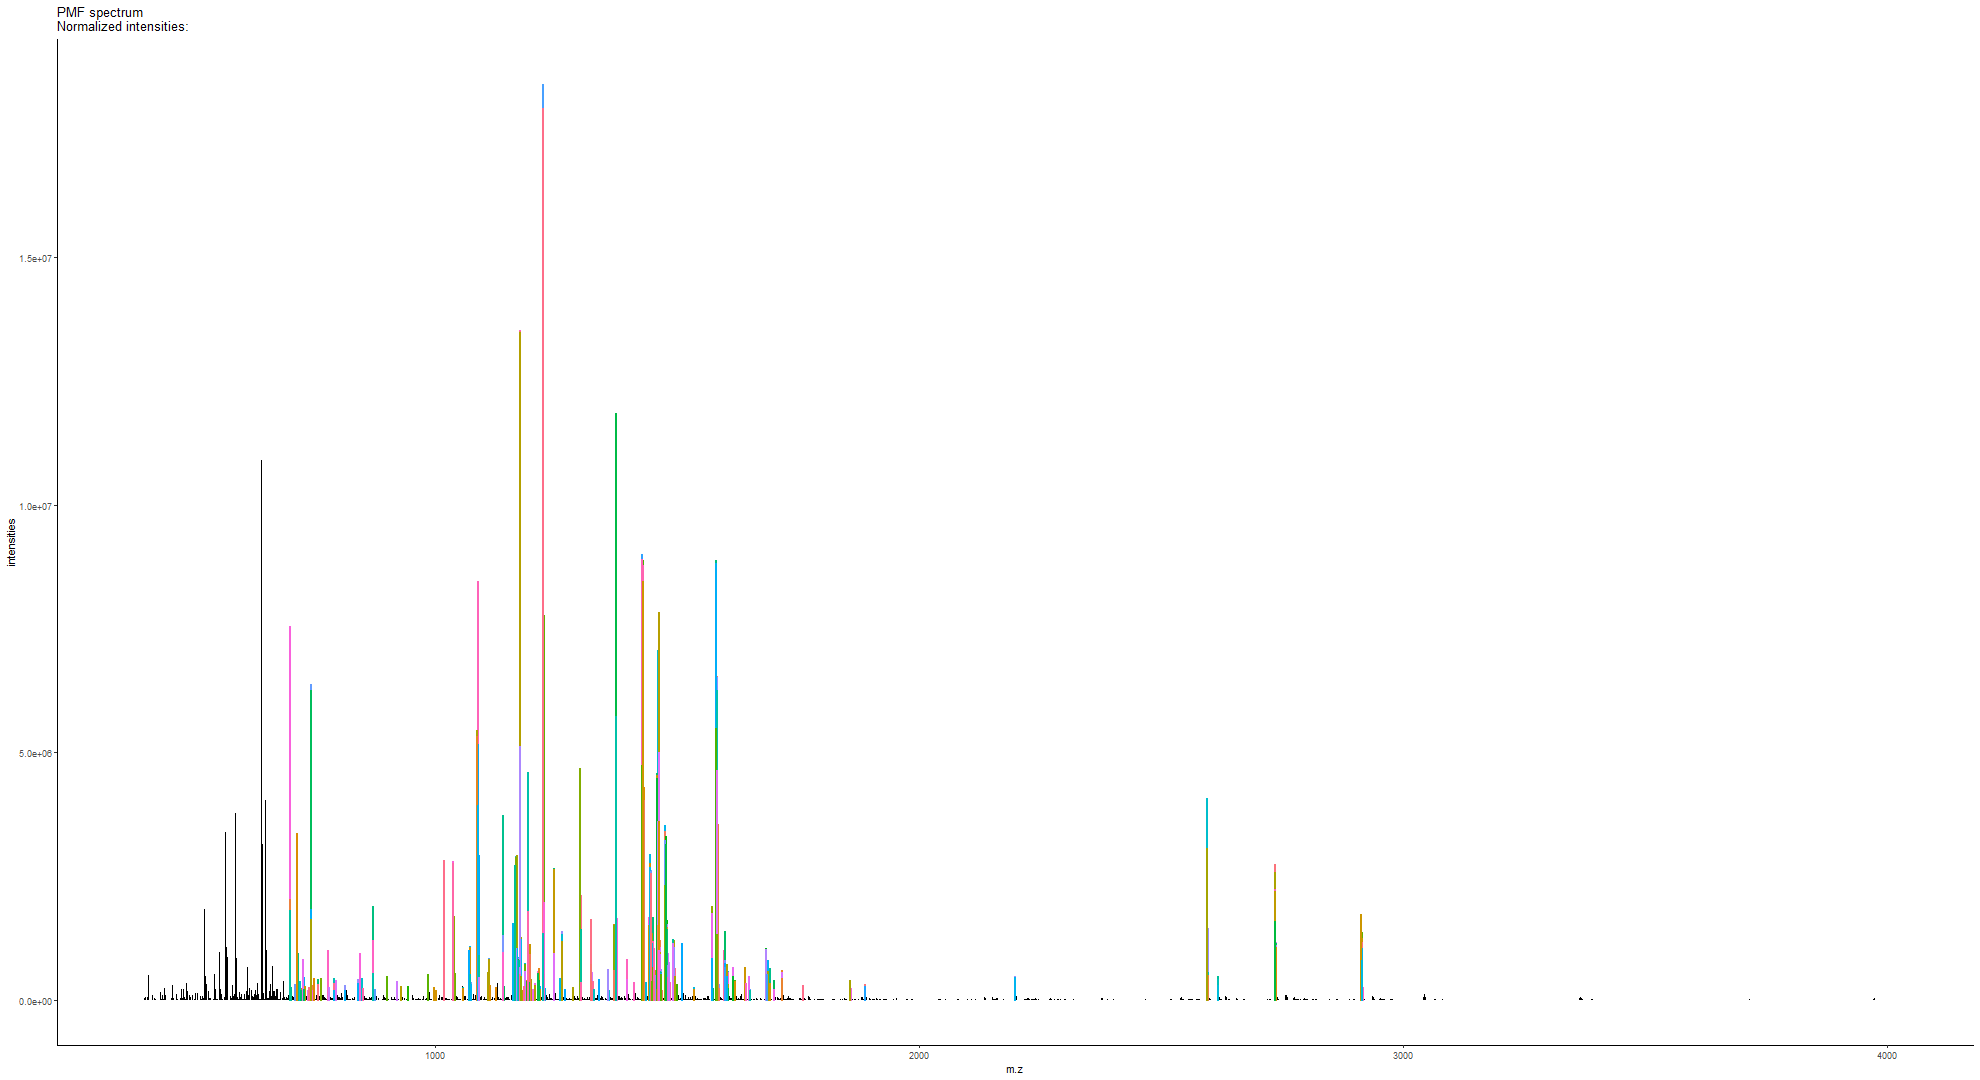
\includegraphics[width=27.5in]{README_files/figure-latex/unnamed-chunk-6-1}

list of Peptides and proteins of each region has also been created so
that you may check each individual region's result.

\begin{Shaded}
\begin{Highlighting}[]
\NormalTok{peptide\_pmf\_result}\OtherTok{\textless{}{-}}\FunctionTok{read.csv}\NormalTok{(}\FunctionTok{paste0}\NormalTok{(wd,datafile,}\StringTok{" ID/Peptide\_segment\_PMF\_RESULT\_3.csv"}\NormalTok{))}
\FunctionTok{head}\NormalTok{(peptide\_pmf\_result)}
\end{Highlighting}
\end{Shaded}

\begin{verbatim}
##   Protein       mz Protein_coverage isdecoy       Peptide Modification    pepmz
## 1      48 1300.664       0.06875544       0   HLEQFATEGLR           NA 1299.657
## 2      48 1300.661       0.06875544       0   QYFLDLALSCK           NA 1299.653
## 3      48 1324.643       0.06875544       0   GSKCILYCFYK           NA 1323.636
## 4      53 1328.747       0.05542725       0   FKNINPFPVPR           NA 1327.740
## 5      53 1449.712       0.05542725       0  AVQNFTEYNVHK           NA 1448.705
## 6      53 1605.813       0.05542725       0 AVQNFTEYNVHKR           NA 1604.806
##          formula adduct charge start end pro_end mz_align      Score Rank
## 1   C57H90N17O18    M+H      1   580 590    1149 1300.666  2.4633527    4
## 2 C60H94N13O17S1    M+H      1   744 754    1149 1300.666  2.0216690   10
## 3 C62H94N13O15S2    M+H      1   840 850    1149 1324.647 -0.2644896   32
## 4   C64H98N17O14    M+H      1   207 217     433 1328.747  1.0865820    7
## 5   C65H97N18O20    M+H      1    92 103     433 1449.714  0.7060553   10
## 6  C71H109N22O21    M+H      1    92 104     433 1605.806  2.7178547   11
##   moleculeNames Region Delta_ppm Intensity peptide_count
## 1   HLEQFATEGLR      3 0.9026772 4672324.6             3
## 2   QYFLDLALSCK      3 1.4117311 4672324.6             3
## 3   GSKCILYCFYK      3 1.5164261  145191.4             3
## 4   FKNINPFPVPR      3 0.9094769  191636.4             3
## 5  AVQNFTEYNVHK      3 2.8830137 1275214.1             3
## 6 AVQNFTEYNVHKR      3 1.6464326  558610.4             3
##                                                                                                                                          desc.x
## 1                                  sp|Q29449|AT8A1_BOVIN Probable phospholipid-transporting ATPase IA OS=Bos taurus OX=9913 GN=ATP8A1 PE=1 SV=2
## 2                                  sp|Q29449|AT8A1_BOVIN Probable phospholipid-transporting ATPase IA OS=Bos taurus OX=9913 GN=ATP8A1 PE=1 SV=2
## 3                                  sp|Q29449|AT8A1_BOVIN Probable phospholipid-transporting ATPase IA OS=Bos taurus OX=9913 GN=ATP8A1 PE=1 SV=2
## 4 sp|Q3SX05|ECSIT_BOVIN Evolutionarily conserved signaling intermediate in Toll pathway, mitochondrial OS=Bos taurus OX=9913 GN=ECSIT PE=2 SV=1
## 5 sp|Q3SX05|ECSIT_BOVIN Evolutionarily conserved signaling intermediate in Toll pathway, mitochondrial OS=Bos taurus OX=9913 GN=ECSIT PE=2 SV=1
## 6 sp|Q3SX05|ECSIT_BOVIN Evolutionarily conserved signaling intermediate in Toll pathway, mitochondrial OS=Bos taurus OX=9913 GN=ECSIT PE=2 SV=1
##                                                                                                                                          desc.y
## 1                                  sp|Q29449|AT8A1_BOVIN Probable phospholipid-transporting ATPase IA OS=Bos taurus OX=9913 GN=ATP8A1 PE=1 SV=2
## 2                                  sp|Q29449|AT8A1_BOVIN Probable phospholipid-transporting ATPase IA OS=Bos taurus OX=9913 GN=ATP8A1 PE=1 SV=2
## 3                                  sp|Q29449|AT8A1_BOVIN Probable phospholipid-transporting ATPase IA OS=Bos taurus OX=9913 GN=ATP8A1 PE=1 SV=2
## 4 sp|Q3SX05|ECSIT_BOVIN Evolutionarily conserved signaling intermediate in Toll pathway, mitochondrial OS=Bos taurus OX=9913 GN=ECSIT PE=2 SV=1
## 5 sp|Q3SX05|ECSIT_BOVIN Evolutionarily conserved signaling intermediate in Toll pathway, mitochondrial OS=Bos taurus OX=9913 GN=ECSIT PE=2 SV=1
## 6 sp|Q3SX05|ECSIT_BOVIN Evolutionarily conserved signaling intermediate in Toll pathway, mitochondrial OS=Bos taurus OX=9913 GN=ECSIT PE=2 SV=1
\end{verbatim}

\begin{Shaded}
\begin{Highlighting}[]
\NormalTok{protein\_pmf\_result}\OtherTok{\textless{}{-}}\FunctionTok{read.csv}\NormalTok{(}\FunctionTok{paste0}\NormalTok{(wd,datafile,}\StringTok{" ID/Protein\_segment\_PMF\_RESULT\_3.csv"}\NormalTok{))}
\FunctionTok{head}\NormalTok{(protein\_pmf\_result)}
\end{Highlighting}
\end{Shaded}

\begin{verbatim}
##   Protein   Proscore isdecoy Intensity     Score peptide_count Protein_coverage
## 1   10134 0.13943597       0 2873903.1 1.9269417             3       0.06715328
## 2   10204 0.13654123       0  380571.3 0.7940642             3       0.18468468
## 3   10370 0.20365140       0 1877250.1 2.0776861             4       0.09364548
## 4   10659 0.11239668       0  327352.4 0.7448240             3       0.16400000
## 5   10888 0.07975644       0  532832.0 1.2420183             3       0.06720978
## 6   11270 0.10687770       0 2944154.2 1.3292158             3       0.07449857
##   Intensity_norm
## 1      1.0775539
## 2      0.9310593
## 3      1.0466962
## 4      0.9201443
## 5      0.9554442
## 6      1.0793038
##                                                                                                                          desc
## 1                   tr|G3N2M8|G3N2M8_BOVIN Sterile alpha motif domain containing 15 OS=Bos taurus OX=9913 GN=SAMD15 PE=4 SV=2
## 2                                      tr|A0A3Q1LYB6|A0A3Q1LYB6_BOVIN Uncharacterized protein OS=Bos taurus OX=9913 PE=4 SV=1
## 3             tr|E1B9U7|E1B9U7_BOVIN Polypeptide N-acetylgalactosaminyltransferase OS=Bos taurus OX=9913 GN=GALNT17 PE=3 SV=3
## 4 tr|A0A3Q1M1B1|A0A3Q1M1B1_BOVIN Phosphatidylinositol transfer protein beta isoform OS=Bos taurus OX=9913 GN=PITPNB PE=4 SV=1
## 5                                  tr|F1MMD4|F1MMD4_BOVIN Matrix metallopeptidase 11 OS=Bos taurus OX=9913 GN=MMP11 PE=3 SV=2
## 6                         tr|F6RR01|F6RR01_BOVIN Ribosome production factor 1 homolog OS=Bos taurus OX=9913 GN=RPF1 PE=4 SV=1
\end{verbatim}

\hypertarget{scoring-system-for-protein-and-peptide}{%
\subsection{Scoring system for protein and
peptide}\label{scoring-system-for-protein-and-peptide}}

\textbf{Score} in peptide result table shows the isotopic pattern
matching score of the peptide (Pepscore). In Protein result table, it
shows the protein score (Proscore). The Pepscore consist of two parts:
Intensity\_Score and Mass\_error\_Score:

\begin{itemize}
\item
  Intensity\_Score indicates how well a putative isotopic pattern can be
  matched to the observed spectrum.The default scoring method is SQRTP.
  It combines the Square root mean differences between observed and
  theoretical peaks and observed proportion of the isotopic peaks above
  a certain relative intensity threshold.
\item
  Mass\_error\_Score indicates the summary of mass error (in \emph{ppm})
  for every detected isotopic peak. in order to integrate the
  Mass\_error\_Score in to scoring system. the mean ppm error has been
  normalized by ppm tolerance, and supplied to the probability normal
  distributions (\emph{pnorm} function for R). The resulting value
  (Quantiles of the given Probability Density) is deducted by 0.5 and
  converted into absolute value.
\end{itemize}

\(Intensity\_Score=\log(PeakCount_{Observed}/PeakCount_{Theoritical})-\log(\sqrt{\frac{\sum_{x = 1}^{n} (Theoritical\_intensity_x-Observed\_intensity_x)^2}{\sum_{x = 1}^{n} (Theoritical\_intensity_x)^2(Observed\_intensity_x)^2}}\)

\(Mass\_error\_Score=|(p\_norm\_dist(\frac{mean\_ppm\_error}{ppm\_tolerance})-0.5)|\)

\(Pepscore=Intensity\_Score-Mass\_error\_Score\)

\textbf{Proscore} in the protein result table shows the overall
estimation of the protein identification Accuracy

\(Proscore=\frac{\sum_{x = 1}^{n}(Pepscore_x*log(Intensity_x))}{mean(log(Intensity))}*Protein\_coverage*Normalized\_intensity\)

A \emph{Peptide\_region\_file.csv} has also been created to summarise
all the IDs in this data file:

\begin{Shaded}
\begin{Highlighting}[]
\NormalTok{Identification\_summary\_table}\OtherTok{\textless{}{-}}\FunctionTok{read.csv}\NormalTok{(}\FunctionTok{paste0}\NormalTok{(wd,datafile,}\StringTok{" ID/Peptide\_region\_file.csv"}\NormalTok{))}
\FunctionTok{head}\NormalTok{(Identification\_summary\_table)}
\end{Highlighting}
\end{Shaded}

\begin{verbatim}
##   Protein        mz Protein_coverage isdecoy              Peptide Modification
## 1      24 1143.5793       0.06119704       0         GFPGQDGLAGPK           NA
## 2      24 1684.8878       0.06119704       0   DGANGIPGPIGPPGPRGR           NA
## 3      24  742.3478       0.06119704       0             GDSGPPGR           NA
## 4      24 1693.8214       0.06119704       0      LLSTEGSQNITYHCK           NA
## 5      24 1881.9276       0.06119704       0 GQPGVMGFPGPKGANGEPGK           NA
## 6      48 1216.7008       0.03481288       0          ASTSVQNRLLK           NA
##       pepmz         formula adduct charge start  end pro_end  mz_align
## 1 1142.5720    C51H79N14O16    M+H      1   516  527    1487 1143.5828
## 2 1683.8805   C72H118N25O22    M+H      1  1175 1192    1487 1684.8830
## 3  741.3406    C29H48N11O12    M+H      1   933  940    1487  742.3504
## 4 1692.8141 C72H117N20O25S1    M+H      1  1380 1394    1487 1693.8197
## 5 1880.9203 C82H129N24O25S1    M+H      1   597  616    1487 1881.9268
## 6 1215.6935    C51H94N17O17    M+H      1   614  624    1149 1216.7047
##       Score Rank        moleculeNames Region Delta_ppm Intensity peptide_count
## 1 1.4443497    2         GFPGQDGLAGPK      2 1.3471596  250698.3             5
## 2 1.9337304    2   DGANGIPGPIGPPGPRGR      2 1.5937657 2696717.3             5
## 3 1.2698949    1             GDSGPPGR      2 0.1407633  190469.7             5
## 4 1.3660521    3      LLSTEGSQNITYHCK      2 2.2329023  368927.9             5
## 5 0.5868561   17 GQPGVMGFPGPKGANGEPGK      2 3.0817671  974427.3             5
## 6 1.9039495    1          ASTSVQNRLLK      2 1.8837090 2036000.7             1
##                                                                                                         desc.x
## 1                   sp|P02459|CO2A1_BOVIN Collagen alpha-1(II) chain OS=Bos taurus OX=9913 GN=COL2A1 PE=1 SV=4
## 2                   sp|P02459|CO2A1_BOVIN Collagen alpha-1(II) chain OS=Bos taurus OX=9913 GN=COL2A1 PE=1 SV=4
## 3                   sp|P02459|CO2A1_BOVIN Collagen alpha-1(II) chain OS=Bos taurus OX=9913 GN=COL2A1 PE=1 SV=4
## 4                   sp|P02459|CO2A1_BOVIN Collagen alpha-1(II) chain OS=Bos taurus OX=9913 GN=COL2A1 PE=1 SV=4
## 5                   sp|P02459|CO2A1_BOVIN Collagen alpha-1(II) chain OS=Bos taurus OX=9913 GN=COL2A1 PE=1 SV=4
## 6 sp|Q29449|AT8A1_BOVIN Probable phospholipid-transporting ATPase IA OS=Bos taurus OX=9913 GN=ATP8A1 PE=1 SV=2
##                                                                                                         desc.y
## 1                   sp|P02459|CO2A1_BOVIN Collagen alpha-1(II) chain OS=Bos taurus OX=9913 GN=COL2A1 PE=1 SV=4
## 2                   sp|P02459|CO2A1_BOVIN Collagen alpha-1(II) chain OS=Bos taurus OX=9913 GN=COL2A1 PE=1 SV=4
## 3                   sp|P02459|CO2A1_BOVIN Collagen alpha-1(II) chain OS=Bos taurus OX=9913 GN=COL2A1 PE=1 SV=4
## 4                   sp|P02459|CO2A1_BOVIN Collagen alpha-1(II) chain OS=Bos taurus OX=9913 GN=COL2A1 PE=1 SV=4
## 5                   sp|P02459|CO2A1_BOVIN Collagen alpha-1(II) chain OS=Bos taurus OX=9913 GN=COL2A1 PE=1 SV=4
## 6 sp|Q29449|AT8A1_BOVIN Probable phospholipid-transporting ATPase IA OS=Bos taurus OX=9913 GN=ATP8A1 PE=1 SV=2
\end{verbatim}

The details of protein/peptide identification process has been save to
the folder named by the segmentation:

\begin{Shaded}
\begin{Highlighting}[]
\FunctionTok{list.dirs}\NormalTok{(}\FunctionTok{paste0}\NormalTok{(wd,datafile,}\StringTok{" ID/"}\NormalTok{), }\AttributeTok{recursive=}\ConstantTok{FALSE}\NormalTok{)}
\end{Highlighting}
\end{Shaded}

\begin{verbatim}
## [1] "D:\\GITHUB LFS\\HiTMaP-Data\\inst/data/Bovinlens_Trypsin_FT/Bovin_lens ID//1"
## [2] "D:\\GITHUB LFS\\HiTMaP-Data\\inst/data/Bovinlens_Trypsin_FT/Bovin_lens ID//2"
## [3] "D:\\GITHUB LFS\\HiTMaP-Data\\inst/data/Bovinlens_Trypsin_FT/Bovin_lens ID//3"
## [4] "D:\\GITHUB LFS\\HiTMaP-Data\\inst/data/Bovinlens_Trypsin_FT/Bovin_lens ID//4"
\end{verbatim}

In the identification details folder, you will find a series of FDR file
and plots to demonstrate the FDR model and score cutoff threshold:

\begin{Shaded}
\begin{Highlighting}[]
\FunctionTok{dir}\NormalTok{(}\FunctionTok{paste0}\NormalTok{(wd,datafile,}\StringTok{" ID/1/"}\NormalTok{), }\AttributeTok{recursive=}\ConstantTok{FALSE}\NormalTok{)}
\end{Highlighting}
\end{Shaded}

\begin{verbatim}
##  [1] "FDR.CSV"                                        
##  [2] "FDR.png"                                        
##  [3] "Matching_Score_vs_mz_target-decoy.png"          
##  [4] "Peptide_1st_ID.csv"                             
##  [5] "Peptide_1st_ID_score_rank_SQRTP.csv"            
##  [6] "Peptide_2nd_ID_score_rankSQRTP_Rank_above_3.csv"
##  [7] "Peptide_Score_histogram_target-decoy.png"       
##  [8] "ppm"                                            
##  [9] "PROTEIN_FDR.CSV"                                
## [10] "Protein_FDR.png"                                
## [11] "Protein_ID_score_rank_SQRTP.csv"                
## [12] "PROTEIN_Score_histogram.png"                    
## [13] "Spectrum.csv"                                   
## [14] "unique_peptide_ranking_vs_mz_feature.png"
\end{verbatim}

In this folder, you will find the FDR plots for protein and peptide. The
software will take the proscore and its FDR model to trim the final
identification result. The
\emph{unique\_peptide\_ranking\_vs\_mz\_feature.png} is a plot that
could tell you the number of peptide candidates have been matched to the
mz features in the first round run.You can also access the peptide
spectrum match (first MS dimension) data via the ``/ppm'' subfolder.

\begin{Shaded}
\begin{Highlighting}[]
\FunctionTok{library}\NormalTok{(magick)}
\NormalTok{p\_peptide\_vs\_mz\_feature}\OtherTok{\textless{}{-}}\FunctionTok{image\_read}\NormalTok{(}\FunctionTok{paste0}\NormalTok{(wd,datafile,}\StringTok{" ID/3/unique\_peptide\_ranking\_vs\_mz\_feature.png"}\NormalTok{))}
\FunctionTok{print}\NormalTok{(p\_peptide\_vs\_mz\_feature)}
\end{Highlighting}
\end{Shaded}

\begin{verbatim}
##   format width height colorspace matte filesize density
## 1    PNG   960    480       sRGB FALSE    11196   72x72
\end{verbatim}

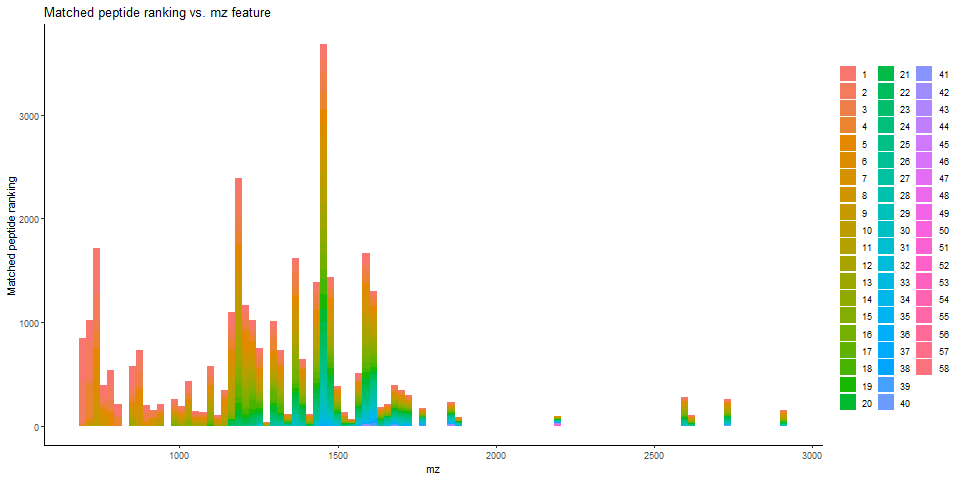
\includegraphics[width=13.33in]{README_files/figure-latex/FDR plot-1}

\begin{Shaded}
\begin{Highlighting}[]
\NormalTok{p\_FDR\_peptide}\OtherTok{\textless{}{-}}\FunctionTok{image\_read}\NormalTok{(}\FunctionTok{paste0}\NormalTok{(wd,datafile,}\StringTok{" ID/3/FDR.png"}\NormalTok{))}
\NormalTok{p\_FDR\_protein}\OtherTok{\textless{}{-}}\FunctionTok{image\_read}\NormalTok{(}\FunctionTok{paste0}\NormalTok{(wd,datafile,}\StringTok{" ID/3/protein\_FDR.png"}\NormalTok{))}
\NormalTok{p\_FDR\_peptide\_his}\OtherTok{\textless{}{-}}\FunctionTok{image\_read}\NormalTok{(}\FunctionTok{paste0}\NormalTok{(wd,datafile,}\StringTok{" ID/3/Peptide\_Score\_histogram\_target{-}decoy.png"}\NormalTok{))}
\NormalTok{p\_FDR\_protein\_his}\OtherTok{\textless{}{-}}\FunctionTok{image\_read}\NormalTok{(}\FunctionTok{paste0}\NormalTok{(wd,datafile,}\StringTok{" ID/3/PROTEIN\_Score\_histogram.png"}\NormalTok{))}
\NormalTok{p\_combined}\OtherTok{\textless{}{-}}\FunctionTok{image\_append}\NormalTok{(}\FunctionTok{c}\NormalTok{(p\_FDR\_peptide,p\_FDR\_peptide\_his,p\_FDR\_protein,p\_FDR\_protein\_his))}
\FunctionTok{print}\NormalTok{(p\_combined)}
\end{Highlighting}
\end{Shaded}

\begin{verbatim}
##   format width height colorspace matte filesize density
## 1    PNG  1920    480       sRGB FALSE        0   72x72
\end{verbatim}

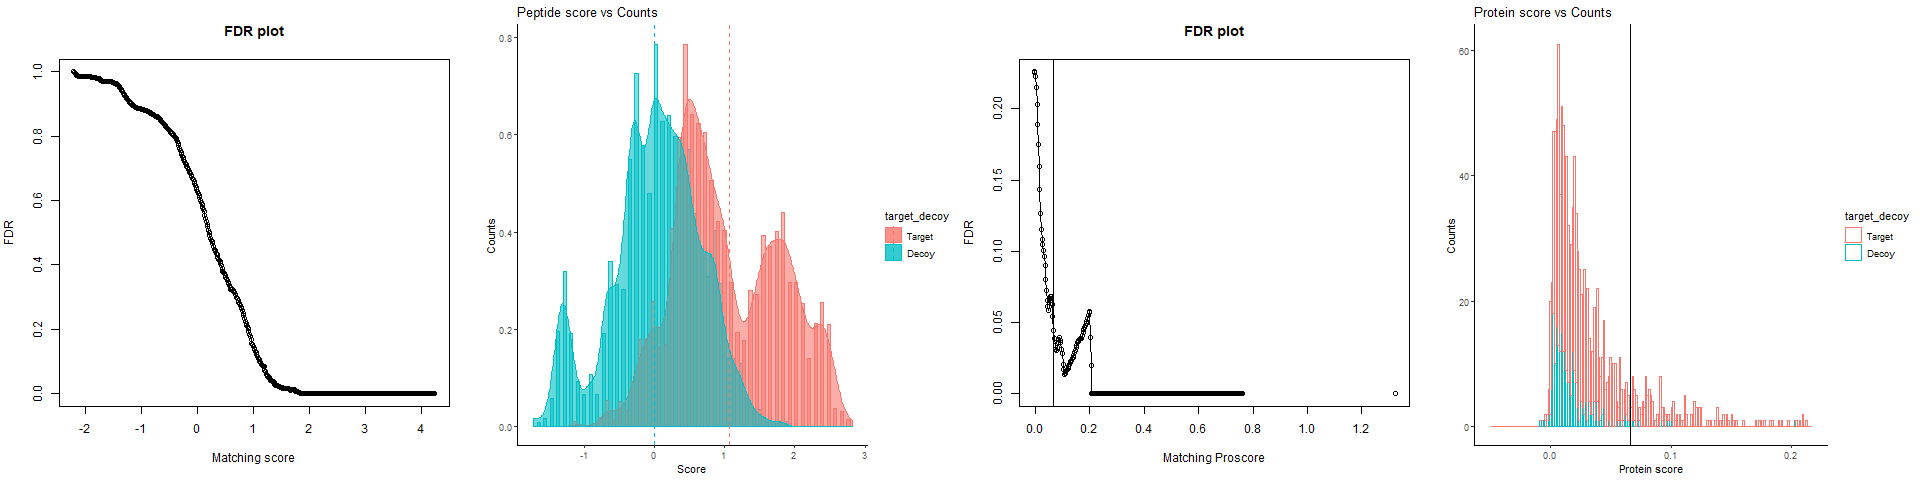
\includegraphics[width=26.67in]{README_files/figure-latex/FDR plot-2}

you will also find a \emph{Matching\_Score\_vs\_mz} plots for further
investigation on peptide matching quality.

\begin{Shaded}
\begin{Highlighting}[]
\FunctionTok{library}\NormalTok{(magick)}
\CommentTok{\#plot Matching\_Score\_vs\_mz}
\NormalTok{p\_Matching\_Score\_vs\_mz}\OtherTok{\textless{}{-}}\FunctionTok{image\_read}\NormalTok{(}\FunctionTok{paste0}\NormalTok{(wd,datafile,}\StringTok{" ID/3/Matching\_Score\_vs\_mz\_target{-}decoy.png"}\NormalTok{))}
\FunctionTok{print}\NormalTok{(p\_Matching\_Score\_vs\_mz)}
\end{Highlighting}
\end{Shaded}

\begin{verbatim}
##   format width height colorspace matte filesize density
## 1    PNG   480    480       sRGB FALSE    47438   72x72
\end{verbatim}

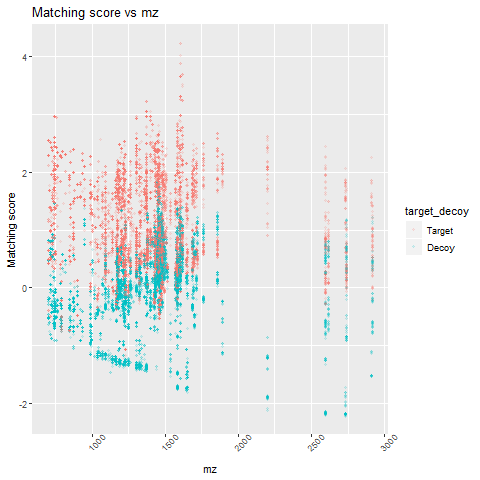
\includegraphics[width=6.67in]{README_files/figure-latex/p_Matching_Score_vs_mz plot-1}

\hypertarget{identification-summary-and-cluster-imaging}{%
\subsection{Identification summary and cluster
imaging}\label{identification-summary-and-cluster-imaging}}

In the project summary folder, you will find four files and a
sub-folder:

\begin{Shaded}
\begin{Highlighting}[]
\NormalTok{wd\_sum}\OtherTok{=}\FunctionTok{paste}\NormalTok{(wd,}\StringTok{"/Summary folder"}\NormalTok{, }\AttributeTok{sep=}\StringTok{""}\NormalTok{)}
\FunctionTok{dir}\NormalTok{(wd\_sum)}
\end{Highlighting}
\end{Shaded}

\begin{verbatim}
## [1] "candidatelist.csv"                "cluster Ion images"              
## [3] "Peptide_Summary.csv"              "Protein_feature_list_trimmed.csv"
## [5] "protein_index.csv"                "Protein_Summary.csv"
\end{verbatim}

``candidatelist.csv'' and ``protein\_index.csv'' contains the candidates
used for this project. They are output after the candidate processing
while \emph{output\_candidatelist} set as TRUE, and can be used
repeatedly while \emph{use\_previous\_candidates} set as TRUE.

we have now implemented a functionality to perform additional
statistical analyses around the number of tryptic enzymatically
generated peptides generated derived from a given proteome
(`Database\_stats'). If the user sets the variable `Database\_stats' to
TRUE in the main workflow, then the function will be called.

Briefly, the function will list all of the m/z's of a unique formulae
from the peptide candidate pool within a given m/z range. The m/z's will
then be binned using three resolution m/z windows: 1ppm, 2ppm and 5ppm.
A plot showing the number of unique formulae vs.~binned m/z windows will
be generated and exported to the summary folder (DB\_stats\_mz\_bin).

The example figure as below shows the m/z bin(s) analysis result of a
mouse brain proteome without modification(s) and with up to 1 missed
cleavage(D). This represents a `worst case scenario' since there is an
assumption that all competitive candidates in each bin have equal
ionisability, which in practice is not the case. The reviewer is
therefore correct that a significant number of competitive candidates
can be found within the m/z range of a common proteomics/peptidomics
investigation. In practical terms, the number of competitive candidates
is likely to be far fewer, due to the previously mentioned unequal
ionisation of predicted peptides and the known bias for MALDI MSI to
detect higher abundance peptides and proteins.

\begin{figure}
\centering
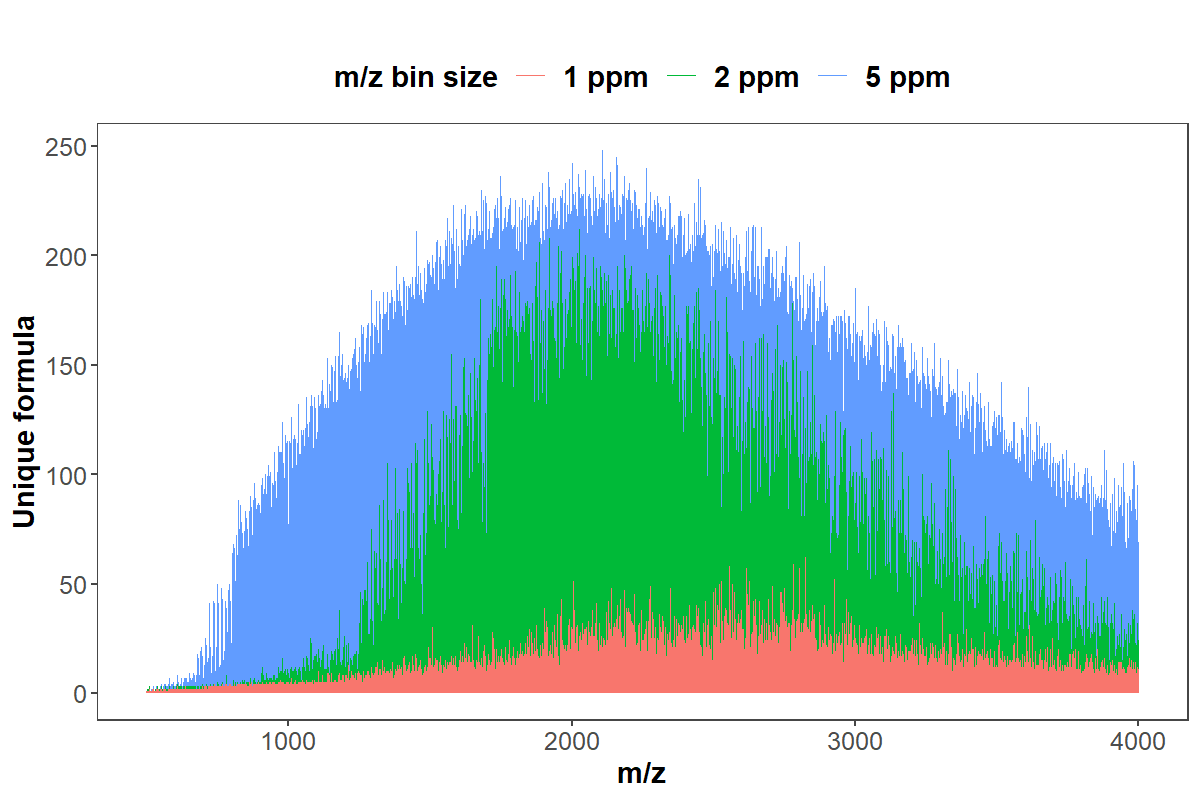
\includegraphics{Resource/DB_stats_bin_mz_ppm.png}
\caption{Proteome database stats}
\end{figure}

However, one of the main applications of HIT-MAP is the annotation of
proteins and their spatial distribution. Since only unique peptides are
retained, and all peptides are rank-scored, and protein maps are only
produced when 2+ unique peptides are matched, we feel that the
likelihood of misidentifying proteins significantly decreases with
increasing peptide number.

``Peptide\_Summary.csv'' and ``Protein\_Summary.csv'' contains the table
of the project identification summary. You could set the
\emph{plot\_cluster\_image\_grid} as TRUE to enable the cluster imaging
function. Please be noted that you could indicate \emph{Rotate\_IMG}
with a CSV file path that indicates the rotation degree of image files.

\textbf{Note}: 90\(^\circ\), 180\(^\circ\) and 270\(^\circ\) are
recommended for image rotation. You may find an example CSV file in the
library/HiTMaP/data folder.

\begin{Shaded}
\begin{Highlighting}[]
\FunctionTok{library}\NormalTok{(dplyr)}
\NormalTok{Protein\_desc\_of\_interest}\OtherTok{\textless{}{-}}\FunctionTok{c}\NormalTok{(}\StringTok{"Crystallin"}\NormalTok{,}\StringTok{"Actin"}\NormalTok{)}
\NormalTok{Protein\_Summary\_tb}\OtherTok{\textless{}{-}}\FunctionTok{read.csv}\NormalTok{(}\FunctionTok{paste}\NormalTok{(wd,}\StringTok{"/Summary folder"}\NormalTok{,}\StringTok{"/Protein\_Summary.csv"}\NormalTok{, }\AttributeTok{sep=}\StringTok{""}\NormalTok{),}\AttributeTok{stringsAsFactors =}\NormalTok{ F)}
\end{Highlighting}
\end{Shaded}

Now you could visualized the interest proteins and their associated
peptides' distribution via cluster imaging function.

\begin{Shaded}
\begin{Highlighting}[]
\FunctionTok{library}\NormalTok{(magick)}
\NormalTok{p\_cluster1}\OtherTok{\textless{}{-}}\FunctionTok{image\_read}\NormalTok{(}\FunctionTok{paste0}\NormalTok{(wd,}\StringTok{"/Summary folder/cluster Ion images/791\_cluster\_imaging.png"}\NormalTok{))}
\FunctionTok{print}\NormalTok{(p\_cluster1)}
\end{Highlighting}
\end{Shaded}

\begin{verbatim}
## # A tibble: 1 x 7
##   format width height colorspace matte filesize density
##   <chr>  <int>  <int> <chr>      <lgl>    <int> <chr>  
## 1 PNG     1980   1308 sRGB       TRUE    302087 118x118
\end{verbatim}

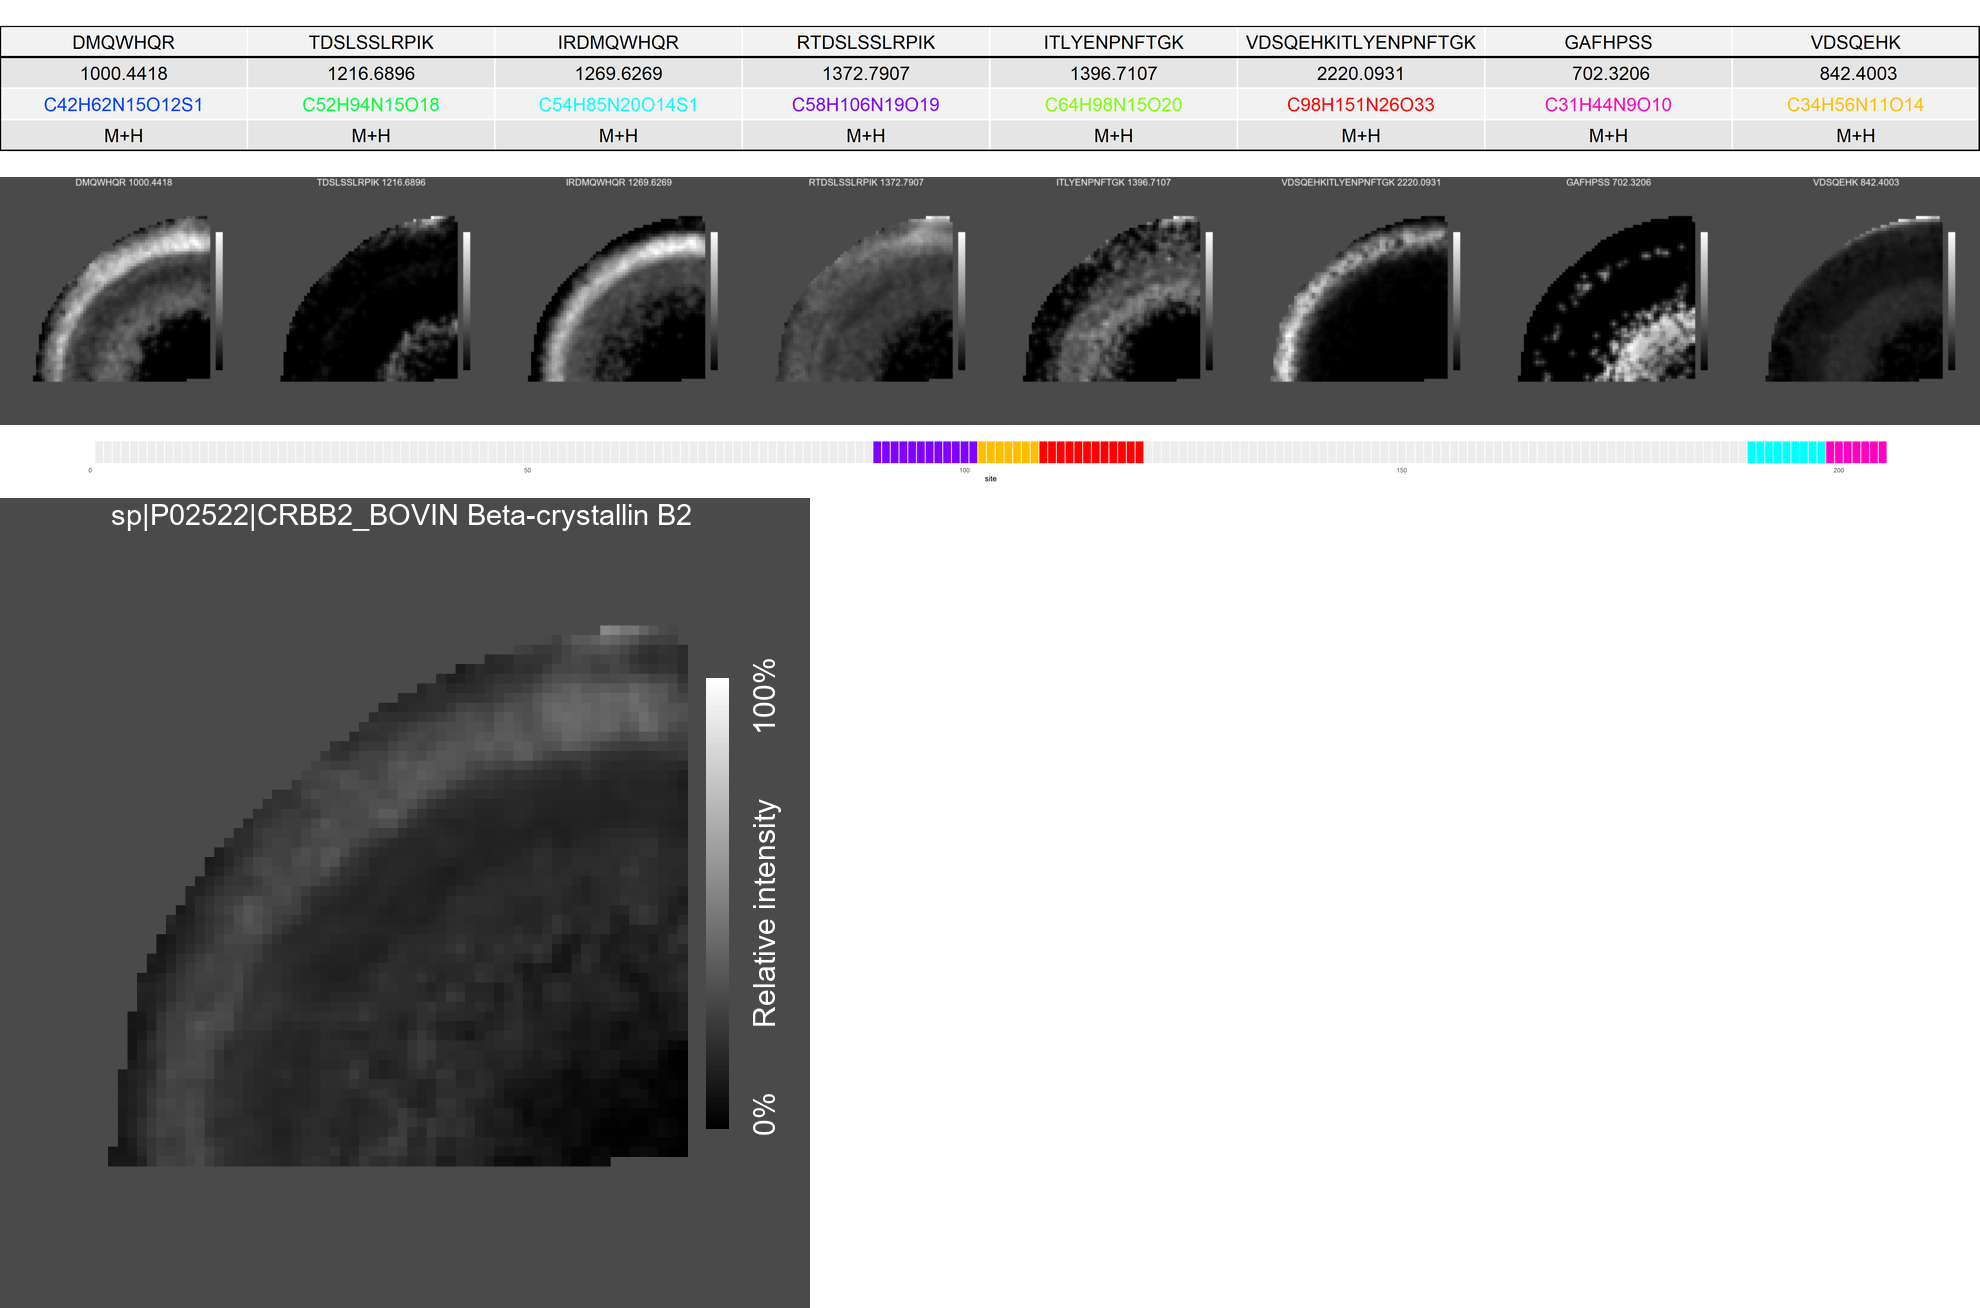
\includegraphics[width=27.5in]{README_files/figure-latex/CLuster imaging-1}

\begin{Shaded}
\begin{Highlighting}[]
\NormalTok{p\_cluster2}\OtherTok{\textless{}{-}}\FunctionTok{image\_read}\NormalTok{(}\FunctionTok{paste0}\NormalTok{(wd,}\StringTok{"/Summary folder/cluster Ion images/5027\_cluster\_imaging.png"}\NormalTok{))}
\FunctionTok{print}\NormalTok{(p\_cluster2)}
\end{Highlighting}
\end{Shaded}

\begin{verbatim}
## # A tibble: 1 x 7
##   format width height colorspace matte filesize density
##   <chr>  <int>  <int> <chr>      <lgl>    <int> <chr>  
## 1 PNG     1980   1309 sRGB       TRUE    348111 118x118
\end{verbatim}

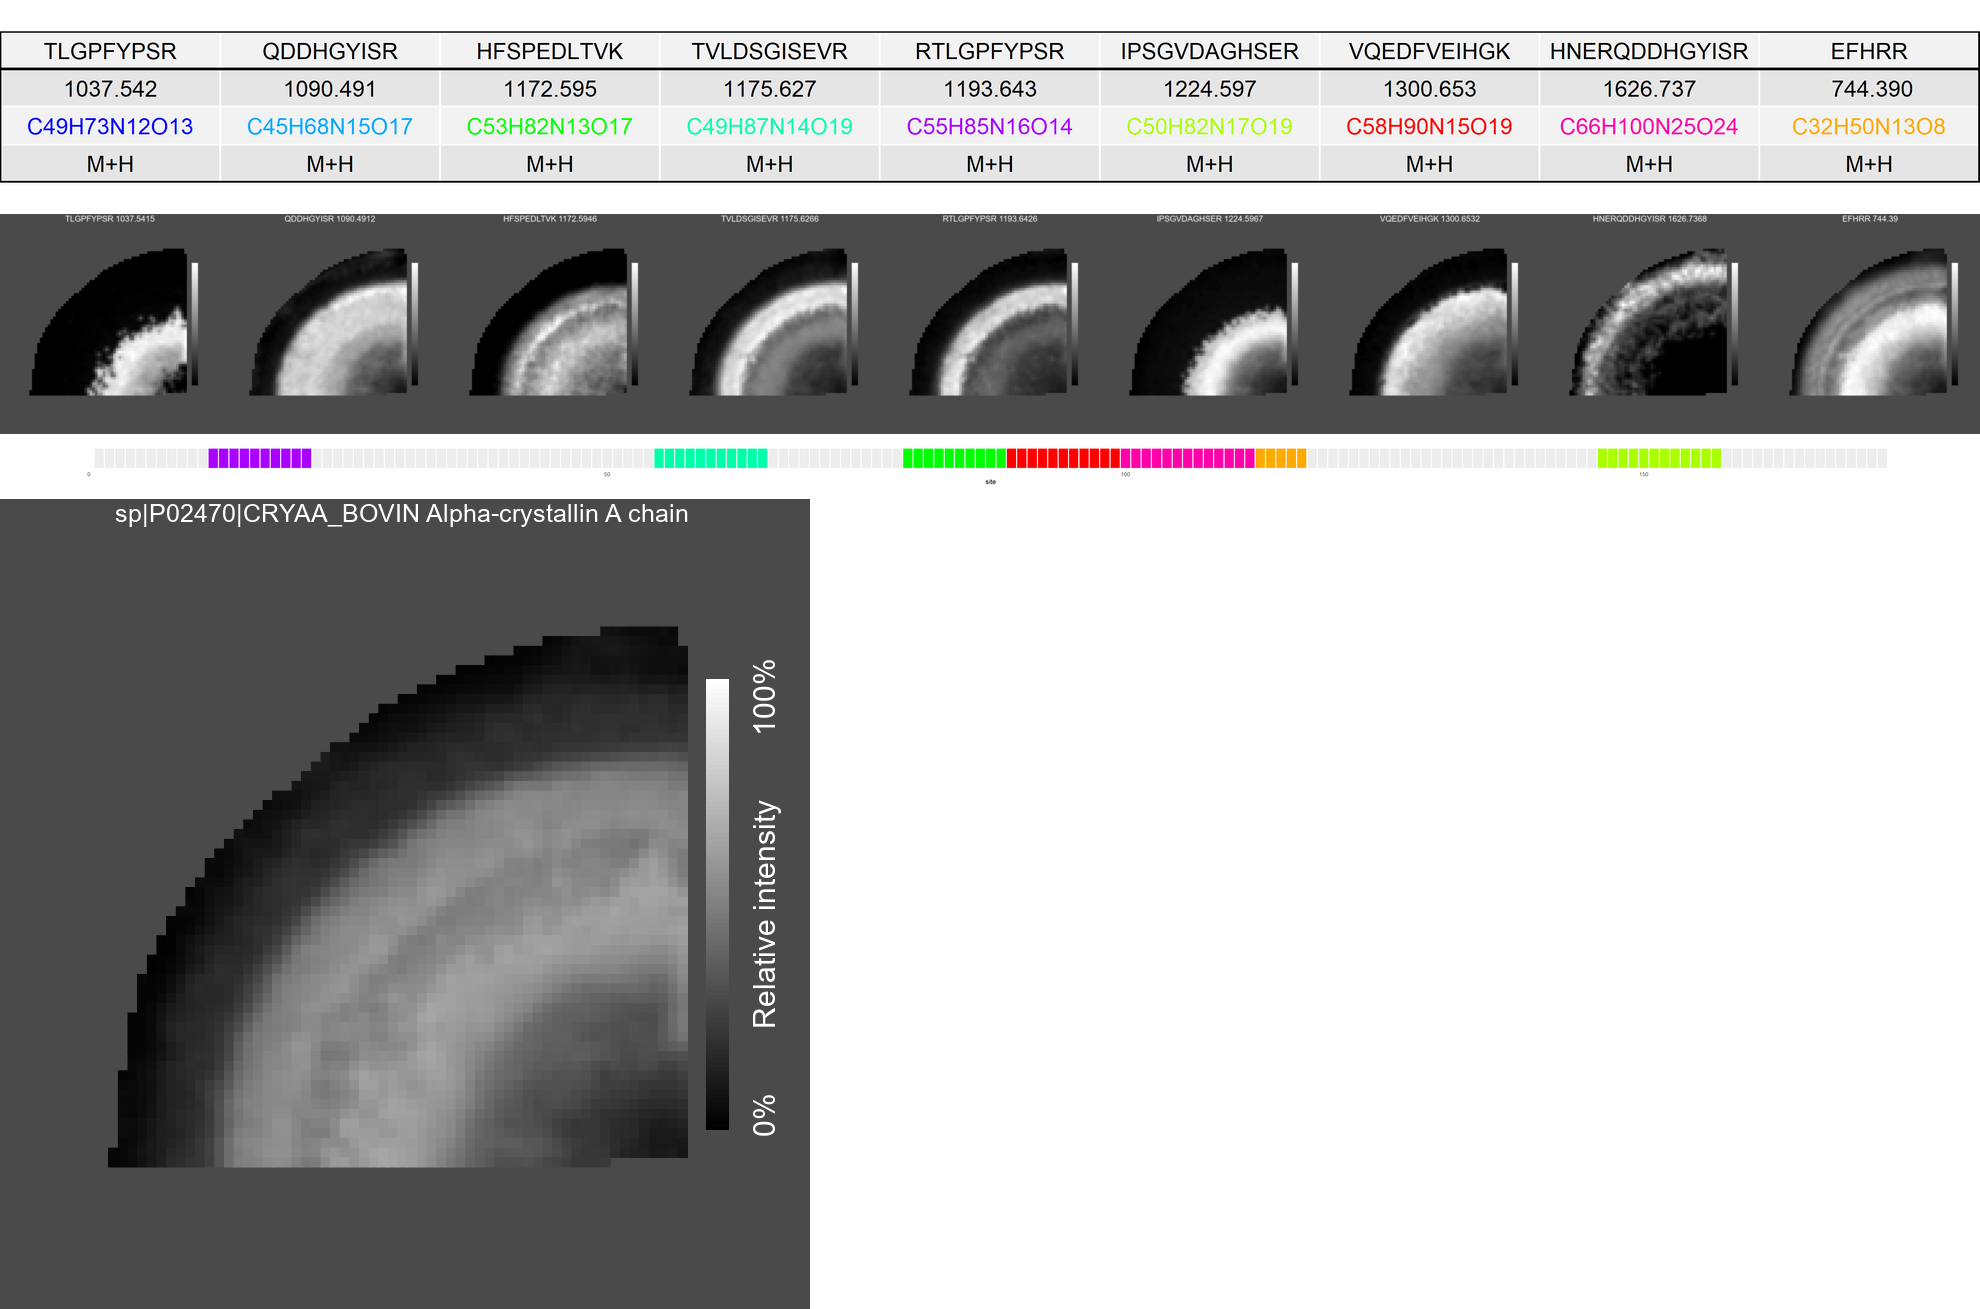
\includegraphics[width=27.5in]{README_files/figure-latex/CLuster imaging-2}

\begin{Shaded}
\begin{Highlighting}[]
\NormalTok{p\_cluster3}\OtherTok{\textless{}{-}}\FunctionTok{image\_read}\NormalTok{(}\FunctionTok{paste0}\NormalTok{(wd,}\StringTok{"/Summary folder/cluster Ion images/5479\_cluster\_imaging.png"}\NormalTok{))}
\FunctionTok{print}\NormalTok{(p\_cluster3)}
\end{Highlighting}
\end{Shaded}

\begin{verbatim}
## # A tibble: 1 x 7
##   format width height colorspace matte filesize density
##   <chr>  <int>  <int> <chr>      <lgl>    <int> <chr>  
## 1 PNG     1980   1069 sRGB       TRUE    237191 118x118
\end{verbatim}

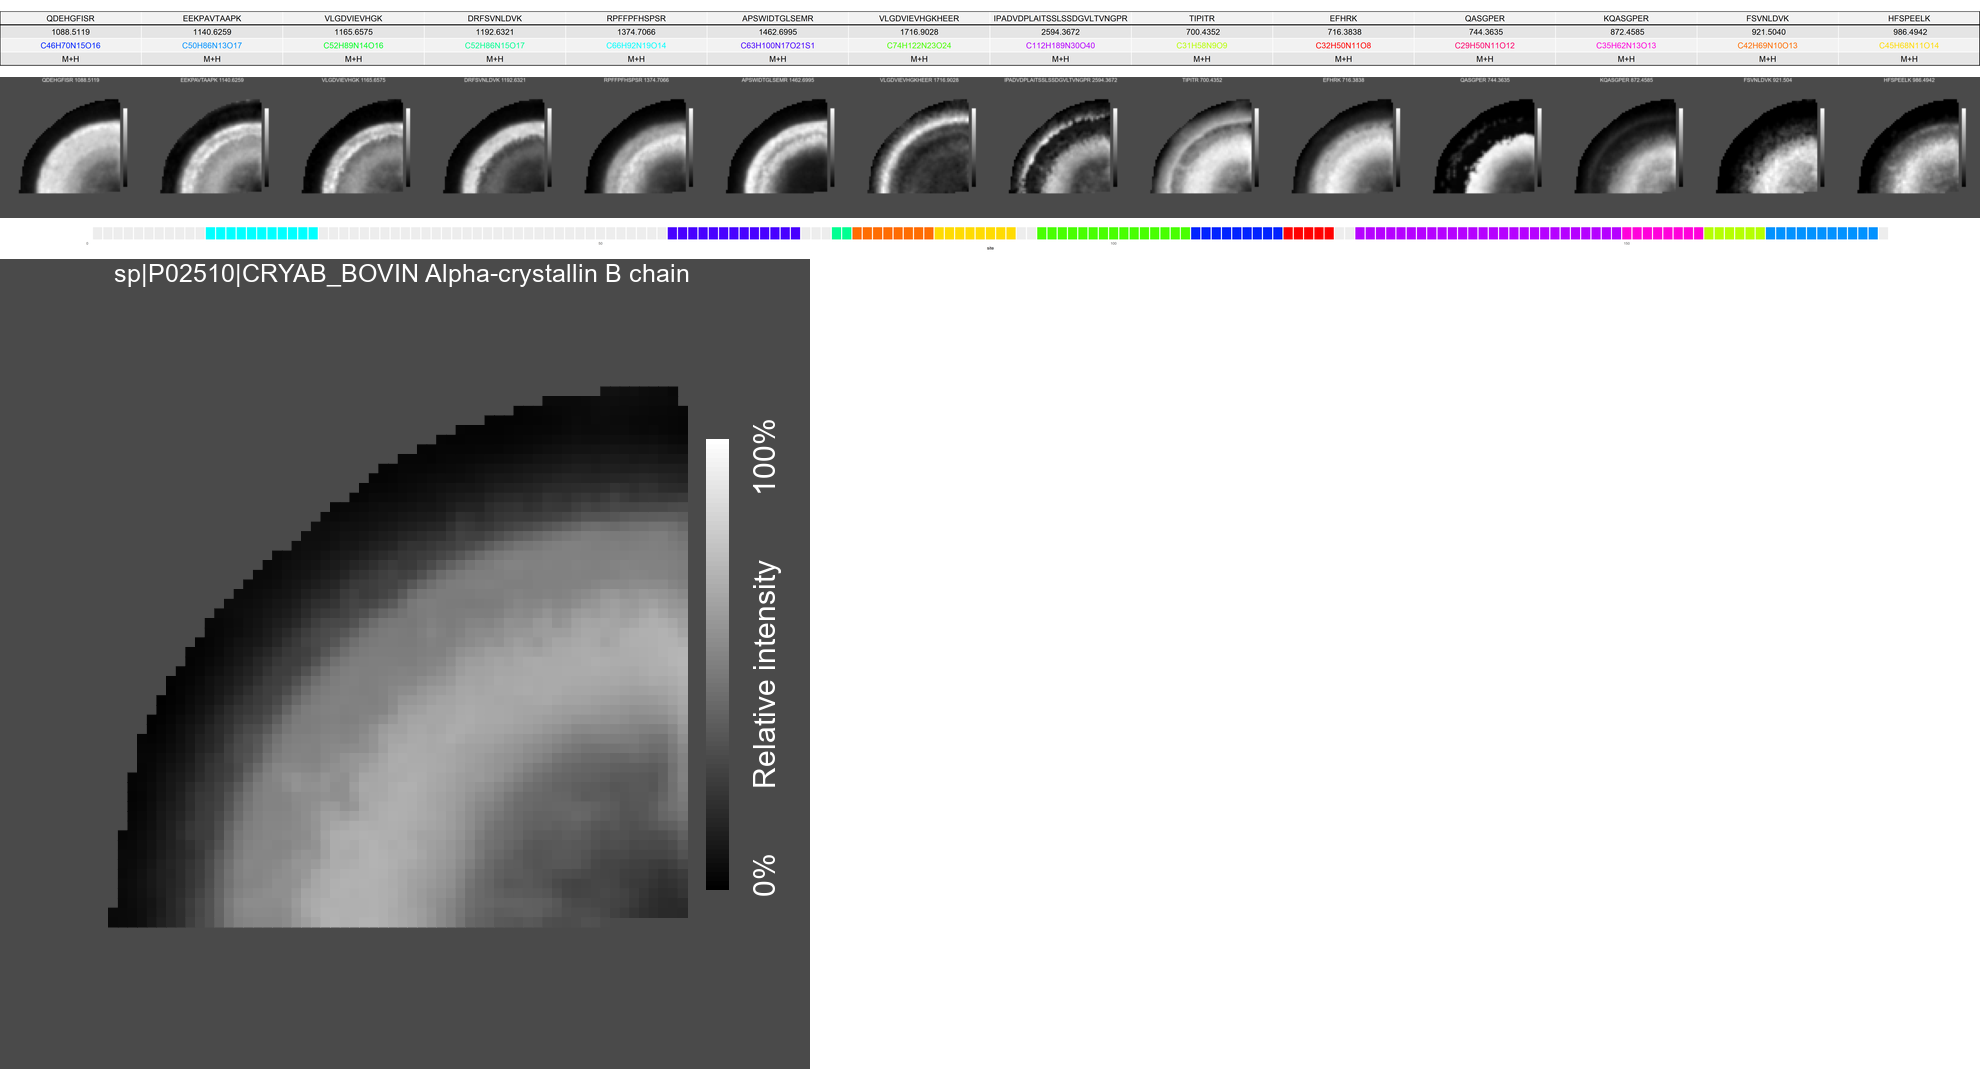
\includegraphics[width=27.5in]{README_files/figure-latex/CLuster imaging-3}

\hypertarget{details-of-parameter-setting}{%
\subsection{Details of parameter
setting}\label{details-of-parameter-setting}}

\hypertarget{modification}{%
\subsubsection{Modification}\label{modification}}

you can choose one or a list of modifications from the unimod
modification list. \emph{Peptide\_modification} function is used to
load/rebuild the modification database into the global enviornment of R.
It will be called automatically in the identification work flow. you can
use the \emph{code\_name} or \emph{record\_id} to refer the modification
(see example data ``peptide calibrants'' to find more details). The
pipeline will select the \emph{non-hidden} modifications.

\begin{Shaded}
\begin{Highlighting}[]
\NormalTok{HiTMaP}\SpecialCharTok{:::}\FunctionTok{Peptide\_modification}\NormalTok{(}\AttributeTok{retrive\_ID=}\ConstantTok{NULL}\NormalTok{,}\AttributeTok{update\_unimod=}\NormalTok{F)}
\NormalTok{modification\_list}\OtherTok{\textless{}{-}}\FunctionTok{merge}\NormalTok{(unimod.df}\SpecialCharTok{$}\NormalTok{modifications,unimod.df}\SpecialCharTok{$}\NormalTok{specificity,}\AttributeTok{by.x=}\FunctionTok{c}\NormalTok{(}\StringTok{"record\_id"}\NormalTok{),}\AttributeTok{by.y=}\FunctionTok{c}\NormalTok{(}\StringTok{"mod\_key"}\NormalTok{),}\AttributeTok{all.x=}\NormalTok{T)}
\FunctionTok{head}\NormalTok{(modification\_list[}\StringTok{\textquotesingle{}\&\textquotesingle{}}\NormalTok{(modification\_list}\SpecialCharTok{$}\NormalTok{code\_name}\SpecialCharTok{==}\StringTok{"Phospho"}\NormalTok{,modification\_list}\SpecialCharTok{$}\NormalTok{hidden}\SpecialCharTok{!=}\DecValTok{1}\NormalTok{),}\FunctionTok{c}\NormalTok{(}\StringTok{"code\_name"}\NormalTok{,}\StringTok{"record\_id"}\NormalTok{,}\StringTok{"composition"}\NormalTok{,}\StringTok{"mono\_mass"}\NormalTok{,}\StringTok{"position\_key"}\NormalTok{,}\StringTok{"one\_letter"}\NormalTok{)])}
\end{Highlighting}
\end{Shaded}

\begin{verbatim}
##      code_name record_id composition mono_mass position_key one_letter
## 1615   Phospho        21    H O(3) P 79.966331            2          Y
## 1618   Phospho        21    H O(3) P 79.966331            2          T
## 1620   Phospho        21    H O(3) P 79.966331            2          S
\end{verbatim}

\begin{Shaded}
\begin{Highlighting}[]
\FunctionTok{head}\NormalTok{(modification\_list[}\StringTok{\textquotesingle{}\&\textquotesingle{}}\NormalTok{(modification\_list}\SpecialCharTok{$}\NormalTok{code\_name}\SpecialCharTok{==}\StringTok{"Amide"}\NormalTok{,modification\_list}\SpecialCharTok{$}\NormalTok{hidden}\SpecialCharTok{!=}\DecValTok{1}\NormalTok{),}\FunctionTok{c}\NormalTok{(}\StringTok{"code\_name"}\NormalTok{,}\StringTok{"record\_id"}\NormalTok{,}\StringTok{"composition"}\NormalTok{,}\StringTok{"mono\_mass"}\NormalTok{,}\StringTok{"position\_key"}\NormalTok{,}\StringTok{"one\_letter"}\NormalTok{)])}
\end{Highlighting}
\end{Shaded}

\begin{verbatim}
##      code_name record_id composition mono_mass position_key one_letter
## 1552     Amide         2   H N O(-1) -0.984016            6     C-term
## 1553     Amide         2   H N O(-1) -0.984016            4     C-term
\end{verbatim}

\begin{Shaded}
\begin{Highlighting}[]
\FunctionTok{head}\NormalTok{(modification\_list[}\StringTok{\textquotesingle{}\&\textquotesingle{}}\NormalTok{(stringr}\SpecialCharTok{::}\FunctionTok{str\_detect}\NormalTok{(modification\_list}\SpecialCharTok{$}\NormalTok{code\_name,}\StringTok{"Ca"}\NormalTok{),modification\_list}\SpecialCharTok{$}\NormalTok{hidden}\SpecialCharTok{!=}\DecValTok{1}\NormalTok{),}\FunctionTok{c}\NormalTok{(}\StringTok{"code\_name"}\NormalTok{,}\StringTok{"record\_id"}\NormalTok{,}\StringTok{"composition"}\NormalTok{,}\StringTok{"mono\_mass"}\NormalTok{,}\StringTok{"position\_key"}\NormalTok{,}\StringTok{"one\_letter"}\NormalTok{)])}
\end{Highlighting}
\end{Shaded}

\begin{verbatim}
##            code_name record_id    composition mono_mass position_key one_letter
## 1946 Carbamidomethyl         4  H(3) C(2) N O 57.021464            2          C
## 1949 Carbamidomethyl         4  H(3) C(2) N O 57.021464            3     N-term
## 2119        Carbamyl         5        H C N O 43.005814            3     N-term
## 2121        Carbamyl         5        H C N O 43.005814            2          K
## 2271   Carboxymethyl         6 H(2) C(2) O(2) 58.005479            2          C
\end{verbatim}

If a modification occurs on different types of site , you will also need
to specify the position of a modifications.

\begin{itemize}
\tightlist
\item
  \emph{Anywhere}, side chain of possible amino acids
\item
  \emph{Any N-term}, any N-term of enzymatic peptide
\item
  \emph{Protein N-term}, any N-term of protein
\end{itemize}

\begin{Shaded}
\begin{Highlighting}[]
\NormalTok{unimod.df[[}\StringTok{"positions"}\NormalTok{]]}
\end{Highlighting}
\end{Shaded}

\begin{verbatim}
##         position record_id
## 1              -         1
## 2       Anywhere         2
## 3     Any N-term         3
## 4     Any C-term         4
## 5 Protein N-term         5
## 6 Protein C-term         6
\end{verbatim}

\hypertarget{amino-acid-substitution}{%
\subsubsection{Amino acid substitution}\label{amino-acid-substitution}}

You can set the \emph{Substitute\_AA} to make the uncommon amino acid
available to the workflow:
\emph{Substitute\_AA=list(AA=c(``X''),AA\_new\_formula=c(``C5H5NO2''),Formula\_with\_water=c(FALSE))}

\begin{itemize}
\tightlist
\item
  AA: the single letter amino acid to be replaced
\item
  AA\_new\_formula: the new formula for the amino acid
\item
  Formula\_with\_water: Set \emph{TRUE} to indicate the formula
  represents the intact amino acid, \emph{FALSE} to indicate that the
  formula already lost one H2O molecule and can be considered as AA
  backbone.
\end{itemize}

\hypertarget{digestion-site-and-enzyme}{%
\subsubsection{Digestion site and
enzyme}\label{digestion-site-and-enzyme}}

The \emph{Digestion\_site} allows you to specify a list of pre-defined
enzyme and customized digestion rules in regular expression format. You
can either use the enzyme name, customized cleavage rule or combination
of them to get the enzymatics peptides list.

\begin{Shaded}
\begin{Highlighting}[]
\NormalTok{Cleavage\_rules}\OtherTok{\textless{}{-}}\FunctionTok{Cleavage\_rules\_fun}\NormalTok{()}
\NormalTok{Cleavage\_df}\OtherTok{\textless{}{-}}\FunctionTok{data.frame}\NormalTok{(}\AttributeTok{Enzyme=}\FunctionTok{names}\NormalTok{(Cleavage\_rules),}\AttributeTok{Cleavage\_rules=}\FunctionTok{unname}\NormalTok{(Cleavage\_rules),}\AttributeTok{stringsAsFactors =}\NormalTok{ F)}
\FunctionTok{library}\NormalTok{(gridExtra)}
\FunctionTok{grid.ftable}\NormalTok{(Cleavage\_df, }\AttributeTok{gp =} \FunctionTok{gpar}\NormalTok{(}\AttributeTok{fontsize=}\DecValTok{9}\NormalTok{,}\AttributeTok{fill =} \FunctionTok{rep}\NormalTok{(}\FunctionTok{c}\NormalTok{(}\StringTok{"grey90"}\NormalTok{, }\StringTok{"grey95"}\NormalTok{))))}
\end{Highlighting}
\end{Shaded}

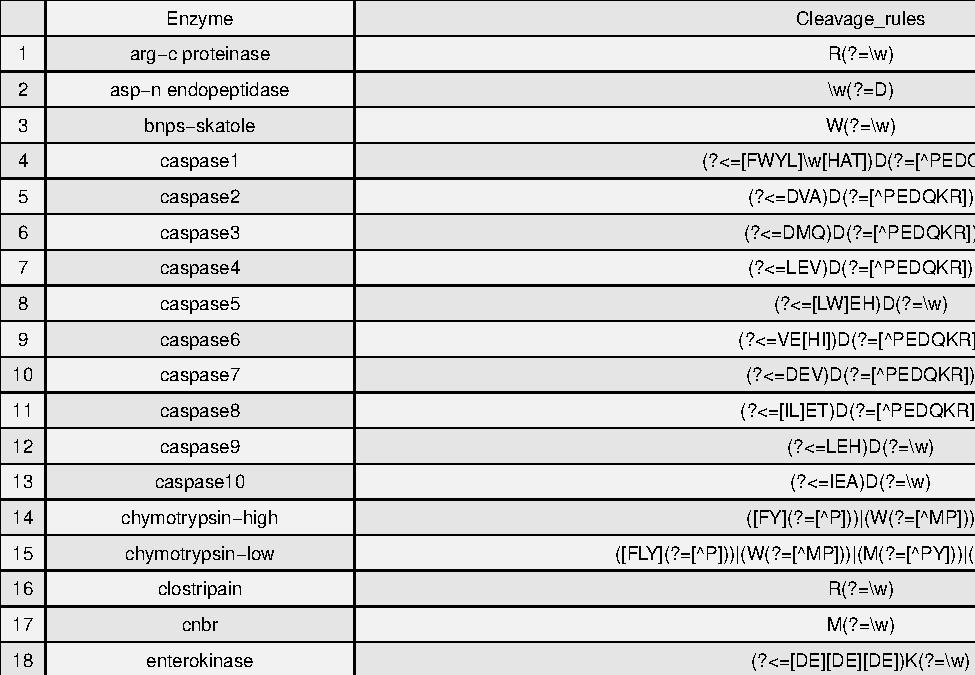
\includegraphics{README_files/figure-latex/unnamed-chunk-13-1.pdf}

\hypertarget{example-workflow-command}{%
\subsection{Example workflow command}\label{example-workflow-command}}

Below is a list of commands including the parameters for the example
data sets.

\hypertarget{peptide-calibrant}{%
\subsubsection{Peptide calibrant}\label{peptide-calibrant}}

\begin{Shaded}
\begin{Highlighting}[]
\CommentTok{\#peptide calibrant}
\FunctionTok{library}\NormalTok{(HiTMaP)}
\NormalTok{datafile}\OtherTok{=}\FunctionTok{c}\NormalTok{(}\StringTok{"Peptide\_calibrants\_FT/trypsin\_non{-}decell\_w.calibrant\_FTICR"}\NormalTok{)}
\NormalTok{wd}\OtherTok{=}\StringTok{"\textasciitilde{}/expdata/"}

\CommentTok{\# Calibrants dataset analysis with modification}
\FunctionTok{imaging\_identification}\NormalTok{(}\AttributeTok{datafile=}\FunctionTok{paste0}\NormalTok{(wd,datafile),}
  \AttributeTok{Digestion\_site=}\StringTok{"trypsin"}\NormalTok{,}
  \AttributeTok{Fastadatabase=}\StringTok{"uniprot\_cali.fasta"}\NormalTok{,}
  \AttributeTok{output\_candidatelist=}\NormalTok{T,}
  \AttributeTok{plot\_matching\_score=}\NormalTok{T,}
  \AttributeTok{spectra\_segments\_per\_file=}\DecValTok{1}\NormalTok{,}
  \AttributeTok{use\_previous\_candidates=}\NormalTok{F,}
  \AttributeTok{peptide\_ID\_filter=}\DecValTok{1}\NormalTok{,}\AttributeTok{ppm=}\DecValTok{5}\NormalTok{,}\AttributeTok{missedCleavages=}\DecValTok{0}\SpecialCharTok{:}\DecValTok{5}\NormalTok{,}
  \AttributeTok{Modifications=}\FunctionTok{list}\NormalTok{(}\AttributeTok{fixed=}\ConstantTok{NULL}\NormalTok{,}\AttributeTok{fixmod\_position=}\ConstantTok{NULL}\NormalTok{,}\AttributeTok{variable=}\FunctionTok{c}\NormalTok{(}\StringTok{"Amide"}\NormalTok{),}\AttributeTok{varmod\_position=}\FunctionTok{c}\NormalTok{(}\DecValTok{6}\NormalTok{)),}
  \AttributeTok{FDR\_cutoff=}\FloatTok{0.1}\NormalTok{,}
  \AttributeTok{Substitute\_AA=}\FunctionTok{list}\NormalTok{(}\AttributeTok{AA=}\FunctionTok{c}\NormalTok{(}\StringTok{"X"}\NormalTok{),}\AttributeTok{AA\_new\_formula=}\FunctionTok{c}\NormalTok{(}\StringTok{"C5H5NO2"}\NormalTok{),}\AttributeTok{Formula\_with\_water=}\FunctionTok{c}\NormalTok{(}\ConstantTok{FALSE}\NormalTok{)))}

\CommentTok{\# Calibrants dataset analysis with no modification}
\FunctionTok{imaging\_identification}\NormalTok{(}\AttributeTok{datafile=}\FunctionTok{paste0}\NormalTok{(wd,datafile),}
  \AttributeTok{Digestion\_site=}\StringTok{"trypsin"}\NormalTok{,}
  \AttributeTok{Fastadatabase=}\StringTok{"uniprot\_cali.fasta"}\NormalTok{,}
  \AttributeTok{output\_candidatelist=}\NormalTok{T,}
  \AttributeTok{plot\_matching\_score=}\NormalTok{T,}
  \AttributeTok{spectra\_segments\_per\_file=}\DecValTok{1}\NormalTok{,}
  \AttributeTok{use\_previous\_candidates=}\NormalTok{T,}
  \AttributeTok{peptide\_ID\_filter=}\DecValTok{1}\NormalTok{,}\AttributeTok{ppm=}\DecValTok{5}\NormalTok{,}\AttributeTok{missedCleavages=}\DecValTok{0}\SpecialCharTok{:}\DecValTok{5}\NormalTok{,}
  \AttributeTok{FDR\_cutoff=}\FloatTok{0.1}\NormalTok{)}

\CommentTok{\# Calibrants dataset analysis with modification }
\FunctionTok{imaging\_identification}\NormalTok{(}\AttributeTok{datafile=}\FunctionTok{paste0}\NormalTok{(wd,datafile),}
  \AttributeTok{Digestion\_site=}\StringTok{"trypsin"}\NormalTok{,}
  \AttributeTok{Fastadatabase=}\StringTok{"calibrants.fasta"}\NormalTok{,}
  \AttributeTok{output\_candidatelist=}\NormalTok{T,}
  \AttributeTok{plot\_matching\_score=}\NormalTok{T,}
  \AttributeTok{spectra\_segments\_per\_file=}\DecValTok{1}\NormalTok{,}
  \AttributeTok{use\_previous\_candidates=}\NormalTok{T,}
  \AttributeTok{peptide\_ID\_filter=}\DecValTok{1}\NormalTok{,}\AttributeTok{ppm=}\DecValTok{5}\NormalTok{,}\AttributeTok{missedCleavages=}\DecValTok{0}\SpecialCharTok{:}\DecValTok{5}\NormalTok{,}
  \AttributeTok{Modifications=}\FunctionTok{list}\NormalTok{(}\AttributeTok{fixed=}\ConstantTok{NULL}\NormalTok{,}\AttributeTok{fixmod\_position=}\ConstantTok{NULL}\NormalTok{,}\AttributeTok{variable=}\FunctionTok{c}\NormalTok{(}\StringTok{"Amide"}\NormalTok{),}\AttributeTok{varmod\_position=}\FunctionTok{c}\NormalTok{(}\DecValTok{6}\NormalTok{)),}
  \AttributeTok{FDR\_cutoff=}\DecValTok{100}\NormalTok{,}
  \AttributeTok{Substitute\_AA=}\FunctionTok{list}\NormalTok{(}\AttributeTok{AA=}\FunctionTok{c}\NormalTok{(}\StringTok{"X"}\NormalTok{),}\AttributeTok{AA\_new\_formula=}\FunctionTok{c}\NormalTok{(}\StringTok{"C5H5NO2"}\NormalTok{),}\AttributeTok{Formula\_with\_water=}\FunctionTok{c}\NormalTok{(}\ConstantTok{FALSE}\NormalTok{)),}\AttributeTok{Thread =} \DecValTok{1}\NormalTok{)}
\end{Highlighting}
\end{Shaded}

\hypertarget{bovin-lens}{%
\subsubsection{Bovin lens}\label{bovin-lens}}

\begin{Shaded}
\begin{Highlighting}[]
\FunctionTok{library}\NormalTok{(HiTMaP)}
\NormalTok{datafile}\OtherTok{=}\FunctionTok{c}\NormalTok{(}\StringTok{"Bovinlens\_Trypsin\_FT/Bovin\_lens.imzML"}\NormalTok{)}
\NormalTok{wd}\OtherTok{=}\StringTok{"\textasciitilde{}/expdata/"}

\CommentTok{\# Data pre{-}processing and proteomics annotation}
\FunctionTok{library}\NormalTok{(HiTMaP)}
\FunctionTok{imaging\_identification}\NormalTok{(}\AttributeTok{datafile=}\FunctionTok{paste0}\NormalTok{(wd,datafile),}\AttributeTok{Digestion\_site=}\StringTok{"trypsin"}\NormalTok{,}
                       \AttributeTok{Fastadatabase=}\StringTok{"uniprot{-}bovin.fasta"}\NormalTok{,}\AttributeTok{output\_candidatelist=}\NormalTok{T,}
                       \AttributeTok{preprocess=}\FunctionTok{list}\NormalTok{(}\AttributeTok{force\_preprocess=}\ConstantTok{TRUE}\NormalTok{,}
                               \AttributeTok{use\_preprocessRDS=}\ConstantTok{TRUE}\NormalTok{,}
                               \AttributeTok{smoothSignal=}\FunctionTok{list}\NormalTok{(}\AttributeTok{method=}\StringTok{"gaussian"}\NormalTok{),}
                               \AttributeTok{reduceBaseline=}\FunctionTok{list}\NormalTok{(}\AttributeTok{method=}\StringTok{"locmin"}\NormalTok{),}
                               \AttributeTok{peakPick=}\FunctionTok{list}\NormalTok{(}\AttributeTok{method=}\StringTok{"adaptive"}\NormalTok{),}
                               \AttributeTok{peakAlign=}\FunctionTok{list}\NormalTok{(}\AttributeTok{tolerance=}\NormalTok{ppm, }\AttributeTok{units=}\StringTok{"ppm"}\NormalTok{),}
                               \AttributeTok{normalize=}\FunctionTok{list}\NormalTok{(}\AttributeTok{method=}\FunctionTok{c}\NormalTok{(}\StringTok{"rms"}\NormalTok{,}\StringTok{"tic"}\NormalTok{,}\StringTok{"reference"}\NormalTok{)[}\DecValTok{1}\NormalTok{],}\AttributeTok{mz=}\DecValTok{1}\NormalTok{)),}
                       \AttributeTok{spectra\_segments\_per\_file=}\DecValTok{9}\NormalTok{,}\AttributeTok{use\_previous\_candidates=}\NormalTok{F,}\AttributeTok{ppm=}\DecValTok{5}\NormalTok{,}\AttributeTok{FDR\_cutoff =} \FloatTok{0.5}\NormalTok{,}\AttributeTok{IMS\_analysis=}\NormalTok{T,}
                       \AttributeTok{Rotate\_IMG=}\StringTok{"file\_rotationbk.csv"}\NormalTok{,}
                       \AttributeTok{mzrange =} \FunctionTok{c}\NormalTok{(}\DecValTok{500}\NormalTok{,}\DecValTok{4000}\NormalTok{),}\AttributeTok{plot\_cluster\_image\_grid=}\NormalTok{F)}

\CommentTok{\# Re{-}analysis and cluster image rendering}

\FunctionTok{library}\NormalTok{(HiTMaP)}
\NormalTok{datafile}\OtherTok{=}\FunctionTok{c}\NormalTok{(}\StringTok{"Bovinlens\_Trypsin\_FT fdr01f/Bovin\_lens.imzML"}\NormalTok{)}
\NormalTok{wd}\OtherTok{=}\StringTok{"\textasciitilde{}/expdata/"}
\FunctionTok{imaging\_identification}\NormalTok{(}\AttributeTok{datafile=}\FunctionTok{paste0}\NormalTok{(wd,datafile),}\AttributeTok{Digestion\_site=}\StringTok{"trypsin"}\NormalTok{,}
                       \AttributeTok{Fastadatabase=}\StringTok{"uniprot{-}bovin.fasta"}\NormalTok{,}
                       \AttributeTok{use\_previous\_candidates=}\NormalTok{T,}\AttributeTok{ppm=}\DecValTok{5}\NormalTok{,}\AttributeTok{IMS\_analysis=}\NormalTok{F,}
                       \AttributeTok{plot\_cluster\_image\_grid=}\NormalTok{T,}
                       \AttributeTok{export\_Header\_table=}\NormalTok{T, }
                       \AttributeTok{img\_brightness=}\DecValTok{250}\NormalTok{, }
                       \AttributeTok{plot\_cluster\_image\_overwrite=}\NormalTok{T,}
                       \AttributeTok{cluster\_rds\_path =} \StringTok{"/Bovin\_lens ID/preprocessed\_imdata.RDS"}\NormalTok{,}\AttributeTok{pixel\_size\_um =} \DecValTok{150}\NormalTok{,}
                       \AttributeTok{Plot\_score\_abs\_cutoff=}\SpecialCharTok{{-}}\FloatTok{0.1}\NormalTok{,}
                       \AttributeTok{remove\_score\_outlier=}\NormalTok{T,}
                       \AttributeTok{Protein\_desc\_of\_interest=}\FunctionTok{c}\NormalTok{(}\StringTok{"Crystallin"}\NormalTok{,}\StringTok{"Phakinin"}\NormalTok{,}\StringTok{"Filensin"}\NormalTok{,}\StringTok{"Actin"}\NormalTok{,}\StringTok{"Vimentin"}\NormalTok{,}\StringTok{"Cortactin"}\NormalTok{,}\StringTok{"Visinin"}\NormalTok{,}\StringTok{"Arpin"}\NormalTok{,}\StringTok{"Tropomyosin"}\NormalTok{,}\StringTok{"Myosin Light Chain 3"}\NormalTok{,}\StringTok{"Kinesin Family Member 14"}\NormalTok{,}\StringTok{"Dynein Regulatory Complex"}\NormalTok{,}\StringTok{"Ankyrin Repeat Domain 45"}\NormalTok{))}
\end{Highlighting}
\end{Shaded}

\hypertarget{mouse-brain}{%
\subsubsection{Mouse brain}\label{mouse-brain}}

\begin{Shaded}
\begin{Highlighting}[]
\FunctionTok{library}\NormalTok{(HiTMaP)}
\NormalTok{datafile}\OtherTok{=}\FunctionTok{c}\NormalTok{(}\StringTok{"MouseBrain\_Trypsin\_FT/Mouse\_brain.imzML"}\NormalTok{)}
\NormalTok{wd}\OtherTok{=}\StringTok{"\textasciitilde{}/expdata/"}

\CommentTok{\# Data pre{-}processing and proteomics annotation}
\FunctionTok{library}\NormalTok{(HiTMaP)}
\FunctionTok{imaging\_identification}\NormalTok{(}\AttributeTok{datafile=}\FunctionTok{paste0}\NormalTok{(wd,datafile),}\AttributeTok{Digestion\_site=}\StringTok{"trypsin"}\NormalTok{,}
                       \AttributeTok{Fastadatabase=}\StringTok{"uniprot\_mouse\_20210107.fasta"}\NormalTok{,}\AttributeTok{output\_candidatelist=}\NormalTok{T,}
                       \AttributeTok{preprocess=}\FunctionTok{list}\NormalTok{(}\AttributeTok{force\_preprocess=}\ConstantTok{TRUE}\NormalTok{,}
                               \AttributeTok{use\_preprocessRDS=}\ConstantTok{TRUE}\NormalTok{,}
                               \AttributeTok{smoothSignal=}\FunctionTok{list}\NormalTok{(}\AttributeTok{method=}\StringTok{"gaussian"}\NormalTok{),}
                               \AttributeTok{reduceBaseline=}\FunctionTok{list}\NormalTok{(}\AttributeTok{method=}\StringTok{"locmin"}\NormalTok{),}
                               \AttributeTok{peakPick=}\FunctionTok{list}\NormalTok{(}\AttributeTok{method=}\StringTok{"adaptive"}\NormalTok{),}
                               \AttributeTok{peakAlign=}\FunctionTok{list}\NormalTok{(}\AttributeTok{tolerance=}\NormalTok{ppm, }\AttributeTok{units=}\StringTok{"ppm"}\NormalTok{),}
                               \AttributeTok{normalize=}\FunctionTok{list}\NormalTok{(}\AttributeTok{method=}\FunctionTok{c}\NormalTok{(}\StringTok{"rms"}\NormalTok{,}\StringTok{"tic"}\NormalTok{,}\StringTok{"reference"}\NormalTok{)[}\DecValTok{1}\NormalTok{],}\AttributeTok{mz=}\DecValTok{1}\NormalTok{)),}
                       \AttributeTok{spectra\_segments\_per\_file=}\DecValTok{9}\NormalTok{,}\AttributeTok{use\_previous\_candidates=}\NormalTok{F,}\AttributeTok{ppm=}\DecValTok{5}\NormalTok{,}\AttributeTok{FDR\_cutoff =} \FloatTok{0.5}\NormalTok{,}\AttributeTok{IMS\_analysis=}\NormalTok{T,}
                       \AttributeTok{Rotate\_IMG=}\StringTok{"file\_rotationbk.csv"}\NormalTok{,}
                       \AttributeTok{mzrange =} \FunctionTok{c}\NormalTok{(}\DecValTok{500}\NormalTok{,}\DecValTok{4000}\NormalTok{),}\AttributeTok{plot\_cluster\_image\_grid=}\NormalTok{F)}

\CommentTok{\# Re{-}analysis and cluster image rendering}

\FunctionTok{imaging\_identification}\NormalTok{(}\AttributeTok{datafile=}\FunctionTok{paste0}\NormalTok{(wd,datafile),}\AttributeTok{Digestion\_site=}\StringTok{"trypsin"}\NormalTok{,}
                       \AttributeTok{Fastadatabase=}\StringTok{"uniprot\_mouse\_20210107.fasta"}\NormalTok{,}
                       \AttributeTok{preprocess=}\FunctionTok{list}\NormalTok{(}\AttributeTok{force\_preprocess=}\ConstantTok{FALSE}\NormalTok{),}
                       \AttributeTok{spectra\_segments\_per\_file=}\DecValTok{9}\NormalTok{,}\AttributeTok{use\_previous\_candidates=}\NormalTok{T,}\AttributeTok{ppm=}\DecValTok{5}\NormalTok{,}\AttributeTok{FDR\_cutoff =} \FloatTok{0.5}\NormalTok{,}\AttributeTok{IMS\_analysis=}\NormalTok{F,}
                       \AttributeTok{mzrange =} \FunctionTok{c}\NormalTok{(}\DecValTok{500}\NormalTok{,}\DecValTok{4000}\NormalTok{),}\AttributeTok{plot\_cluster\_image\_grid=}\NormalTok{T,}
                       \AttributeTok{img\_brightness=}\DecValTok{250}\NormalTok{, }\AttributeTok{plot\_cluster\_image\_overwrite=}\NormalTok{T,}
                       \AttributeTok{cluster\_rds\_path =} \StringTok{"/Mouse\_brain ID/preprocessed\_imdata.RDS"}\NormalTok{,}
                       \AttributeTok{pixel\_size\_um =} \DecValTok{150}\NormalTok{,}
                       \AttributeTok{Plot\_score\_abs\_cutoff=}\SpecialCharTok{{-}}\FloatTok{0.1}\NormalTok{,}
                       \AttributeTok{remove\_score\_outlier=}\NormalTok{T,}
                       \AttributeTok{Protein\_desc\_of\_interest=}\FunctionTok{c}\NormalTok{(}\StringTok{"Crystallin"}\NormalTok{,}\StringTok{"Phakinin"}\NormalTok{,}\StringTok{"Filensin"}\NormalTok{,}\StringTok{"Actin"}\NormalTok{,}\StringTok{"Vimetin"}\NormalTok{,}\StringTok{"Cortactin"}\NormalTok{,}\StringTok{"Visinin"}\NormalTok{,}\StringTok{"Arpin"}\NormalTok{,}\StringTok{"Tropomyosin"}\NormalTok{,}\StringTok{"Myosin Light Chain 3"}\NormalTok{,}\StringTok{"Kinesin Family Member 14"}\NormalTok{,}\StringTok{"Dyenin Regulatory Complex"}\NormalTok{,}\StringTok{"Ankyrin Repeat Domain 45"}\NormalTok{))}
\end{Highlighting}
\end{Shaded}

\hypertarget{session-information}{%
\subsection{Session information}\label{session-information}}

\begin{Shaded}
\begin{Highlighting}[]
\FunctionTok{toLatex}\NormalTok{(}\FunctionTok{sessionInfo}\NormalTok{())}
\end{Highlighting}
\end{Shaded}

\begin{verbatim}
## \begin{itemize}\raggedright
##   \item R version 4.0.2 (2020-06-22), \verb|x86_64-w64-mingw32|
##   \item Locale: \verb|LC_COLLATE=English_Australia.1252|, \verb|LC_CTYPE=English_Australia.1252|, \verb|LC_MONETARY=English_Australia.1252|, \verb|LC_NUMERIC=C|, \verb|LC_TIME=English_Australia.1252|
##   \item Running under: \verb|Windows 10 x64 (build 19042)|
##   \item Matrix products: default
##   \item Base packages: base, datasets, graphics, grDevices, grid,
##     methods, stats, utils
##   \item Other packages: data.table~1.13.6, dplyr~1.0.2, gridExtra~2.3,
##     HiTMaP~1.6.0, lattice~0.20-41, magick~2.5.2, pls~2.7-3,
##     protViz~0.6.8, XML~3.99-0.5
##   \item Loaded via a namespace (and not attached): assertthat~0.2.1,
##     Biobase~2.48.0, BiocGenerics~0.34.0, BiocManager~1.30.10,
##     BiocParallel~1.22.0, cli~2.3.0, codetools~0.2-18, compiler~4.0.2,
##     crayon~1.4.0, digest~0.6.27, ellipsis~0.3.1, evaluate~0.14,
##     fansi~0.4.2, fastmap~1.1.0, generics~0.1.0, glue~1.4.2,
##     gtable~0.3.0, htmltools~0.5.1.1, httpuv~1.5.5, knitr~1.30,
##     later~1.1.0.1, lifecycle~0.2.0, magrittr~2.0.1, MASS~7.3-53,
##     Matrix~1.3-2, mime~0.9, multtest~2.44.0, pacman~0.5.1,
##     parallel~4.0.2, pillar~1.4.7, pkgconfig~2.0.3, png~0.1-7,
##     promises~1.1.1, purrr~0.3.4, R6~2.5.0, Rcpp~1.0.6, rlang~0.4.10,
##     rmarkdown~2.6, S4Vectors~0.26.1, shiny~1.6.0, splines~4.0.2,
##     stats4~4.0.2, stringi~1.5.3, stringr~1.4.0, survival~3.2-7,
##     tibble~3.0.6, tidyselect~1.1.0, tools~4.0.2, utf8~1.1.4,
##     vctrs~0.3.6, xfun~0.20, xtable~1.8-4, yaml~2.2.1
## \end{itemize}
\end{verbatim}

End of the tutorial, Enjoy\textasciitilde{}

\hypertarget{references}{%
\subsection{References}\label{references}}

R Packages used in this project:

\begin{itemize}
\item
  viridisLite(Garnier 2018)
\item
  rcdklibs(Guha 2017)
\item
  rJava(Urbanek 2019)
\item
  data.table(Dowle and Srinivasan 2019)
\item
  RColorBrewer(Neuwirth 2014)
\item
  magick(Ooms 2019)
\item
  ggplot2(Wickham 2016)
\item
  dplyr(Wickham et al. 2019)
\item
  stringr(Wickham 2019)
\item
  protViz(Panse and Grossmann 2019)
\item
  cleaver(Gibb 2019)
\item
  Biostrings(Pag�s et al. 2019)
\item
  IRanges(Lawrence et al. 2013)
\item
  Cardinal(Bemis et al. 2015)
\item
  tcltk(R Core Team 2019)
\item
  BiocParallel(Morgan et al. 2019)
\item
  spdep(Bivand and Wong 2018)
\item
  FTICRMS(Barkauskas 2012)
\item
  UniProt.ws(Carlson 2019)
\end{itemize}

\hypertarget{refs}{}
\begin{CSLReferences}{1}{0}
\leavevmode\hypertarget{ref-FTICRMS}{}%
Barkauskas, Don. 2012. \emph{FTICRMS: Programs for Analyzing Fourier
Transform-Ion Cyclotron Resonance Mass Spectrometry Data}.
\url{https://CRAN.R-project.org/package=FTICRMS}.

\leavevmode\hypertarget{ref-Cardinal}{}%
Bemis, Kyle D., April Harry, Livia S. Eberlin, Christina Ferreira,
Stephanie M. van de Ven, Parag Mallick, Mark Stolowitz, and Olga Vitek.
2015. {``Cardinal: An r Package for Statistical Analysis of Mass
Spectrometry-Based Imaging Experiments.''} \emph{Bioinformatics}.
\url{https://doi.org/10.1093/bioinformatics/btv146}.

\leavevmode\hypertarget{ref-spdep1}{}%
Bivand, Roger, and David W. S. Wong. 2018. {``Comparing Implementations
of Global and Local Indicators of Spatial Association.''} \emph{TEST} 27
(3): 716--48. \url{https://doi.org/10.1007/s11749-018-0599-x}.

\leavevmode\hypertarget{ref-UniProt.ws}{}%
Carlson, Marc. 2019. \emph{UniProt.ws: R Interface to UniProt Web
Services}.

\leavevmode\hypertarget{ref-data.table}{}%
Dowle, Matt, and Arun Srinivasan. 2019. \emph{Data.table: Extension of
`Data.frame`}. \url{https://CRAN.R-project.org/package=data.table}.

\leavevmode\hypertarget{ref-viridisLite}{}%
Garnier, Simon. 2018. \emph{viridisLite: Default Color Maps from
'Matplotlib' (Lite Version)}.
\url{https://CRAN.R-project.org/package=viridisLite}.

\leavevmode\hypertarget{ref-cleaver}{}%
Gibb, Sebastian. 2019. \emph{Cleaver: Cleavage of Polypeptide
Sequences}. \url{https://github.com/sgibb/cleaver/}.

\leavevmode\hypertarget{ref-rcdklibs}{}%
Guha, Rajarshi. 2017. \emph{Rcdklibs: The CDK Libraries Packaged for r}.
\url{https://CRAN.R-project.org/package=rcdklibs}.

\leavevmode\hypertarget{ref-IRanges}{}%
Lawrence, Michael, Wolfgang Huber, Hervé Pagès, Patrick Aboyoun, Marc
Carlson, Robert Gentleman, Martin Morgan, and Vincent Carey. 2013.
{``Software for Computing and Annotating Genomic Ranges.''} \emph{{PLoS}
Computational Biology} 9.
\url{https://doi.org/10.1371/journal.pcbi.1003118}.

\leavevmode\hypertarget{ref-BiocParallel}{}%
Morgan, Martin, Valerie Obenchain, Michel Lang, Ryan Thompson, and
Nitesh Turaga. 2019. \emph{BiocParallel: Bioconductor Facilities for
Parallel Evaluation}.
\url{https://github.com/Bioconductor/BiocParallel}.

\leavevmode\hypertarget{ref-RColorBrewer}{}%
Neuwirth, Erich. 2014. \emph{RColorBrewer: ColorBrewer Palettes}.
\url{https://CRAN.R-project.org/package=RColorBrewer}.

\leavevmode\hypertarget{ref-magick}{}%
Ooms, Jeroen. 2019. \emph{Magick: Advanced Graphics and Image-Processing
in r}. \url{https://CRAN.R-project.org/package=magick}.

\leavevmode\hypertarget{ref-Biostrings}{}%
Pag�s, H., P. Aboyoun, R. Gentleman, and S. DebRoy. 2019.
\emph{Biostrings: Efficient Manipulation of Biological Strings}.

\leavevmode\hypertarget{ref-protViz}{}%
Panse, Christian, and Jonas Grossmann. 2019. \emph{protViz: Visualizing
and Analyzing Mass Spectrometry Related Data in Proteomics}.

\leavevmode\hypertarget{ref-tcltk}{}%
R Core Team. 2019. \emph{R: A Language and Environment for Statistical
Computing}. Vienna, Austria: R Foundation for Statistical Computing.
\url{https://www.R-project.org/}.

\leavevmode\hypertarget{ref-rJava}{}%
Urbanek, Simon. 2019. \emph{rJava: Low-Level r to Java Interface}.
\url{https://CRAN.R-project.org/package=rJava}.

\leavevmode\hypertarget{ref-ggplot2}{}%
Wickham, Hadley. 2016. \emph{Ggplot2: Elegant Graphics for Data
Analysis}. Springer-Verlag New York.
\url{https://ggplot2.tidyverse.org}.

\leavevmode\hypertarget{ref-stringr}{}%
---------. 2019. \emph{Stringr: Simple, Consistent Wrappers for Common
String Operations}. \url{https://CRAN.R-project.org/package=stringr}.

\leavevmode\hypertarget{ref-dplyr}{}%
Wickham, Hadley, Romain Fran�ois, Lionel Henry, and Kirill Muller. 2019.
\emph{Dplyr: A Grammar of Data Manipulation}.
\url{https://CRAN.R-project.org/package=dplyr}.

\end{CSLReferences}

\end{document}
